\documentclass[twoside,twocolumn,10pt]{article}
\usepackage{fancyhdr}
\usepackage{geometry}
\usepackage{multicol}
\usepackage{abstract}
\usepackage{graphicx}
\graphicspath{{imagenes/}}
\usepackage[font=footnotesize, labelfont=bf, justification=raggedright, format=plain]{caption}
\usepackage{subcaption}
\usepackage{threeparttable}
\usepackage{titlesec}
\usepackage{ragged2e}
\usepackage{amssymb}
\usepackage{parskip}
\usepackage{amsmath}
\usepackage{newtxtext}
\usepackage{booktabs}
\usepackage{array}
\usepackage[spanish]{babel}
\usepackage[
	backend=biber,
	style=chem-acs,
	articletitle=false,
	maxnames=4,
	minnames=1
]{biblatex}
\usepackage[version=4]{mhchem}
\usepackage{xurl}
\usepackage{placeins} 
\addbibresource{references.bib}
\setcounter{page}{1}

\renewcommand{\topfraction}{0.85}
\renewcommand{\dbltopfraction}{0.85}
\renewcommand{\textfraction}{0.1}
\renewcommand{\floatpagefraction}{0.75}
\renewcommand{\dblfloatpagefraction}{0.75}
\setlength{\textfloatsep}{12pt plus 2pt minus 2pt}
\setlength{\dbltextfloatsep}{12pt plus 2pt minus 2pt}

\newcolumntype{L}[1]{>{\raggedright\arraybackslash}p{#1}}
\newcolumntype{C}[1]{>{\centering\arraybackslash}p{#1}}
\newcolumntype{R}[1]{>{\raggedleft\arraybackslash}p{#1}}

\captionsetup[table]{labelsep=period, justification=raggedright}
\captionsetup[figure]{labelsep=period, justification=raggedright}

\geometry{letterpaper, left=0.8in, right=0.8in, top=1in, bottom=1in}
\setlength{\columnsep}{20pt}

\renewcommand{\abstractname}{\hspace{1.3em}\textbf{Resumen}}
\titleformat{\section}{\large\bfseries\uppercase}{\thesection.}{1em}{}
\titleformat{\subsection}{\normalfont\bfseries\flushleft}{\thesubsection.}{1em}{}
\titleformat{\subsubsection}{\normalfont\bfseries\itshape\flushleft}{\thesubsubsection}{1em}{}
\renewcommand{\abstractnamefont}{\normalfont\fontsize{14}{20}\bfseries}
\renewcommand{\absnamepos}{flushleft}
\renewcommand{\abstracttextfont}{\normalfont\fontsize{11}{13}\selectfont}

\hyphenpenalty=10000
\exhyphenpenalty=10000
\sloppy

\pagestyle{fancy}
\fancyhf{}
\fancyhead[C]{\small Propiedades y reactividad de diez ácidos carboxílicos}
\fancyhead[CE]{\small Proyecto de Química Orgánica (2026)}
\fancyfoot[C]{\thepage}

\fancypagestyle{firstpage}{
  \fancyhf{}
  \fancyhead[LO]{\small Ingeniería Ambiental, FAMARENA-UD}
  \fancyhead[RO]{\small QUIMORG 2026-III}

  \fancyfoot[R]{\footnotesize \copyright\ 2026, para proyecto final}
  \renewcommand{\headrulewidth}{0.4pt}
  \renewcommand{\footrulewidth}{0.4pt}
}

\title{\fontsize{16}{20}\selectfont\textbf{Proyecto final: análisis de reacciones y obtenciones registradas en CAS SciFinder para 10 ácidos}}

\author{
    \fontsize{12}{14}\selectfont
    Luna Vanessa Guerrero Urrego\textsuperscript{}, Andrea Jiménez Rodríguez\textsuperscript{}, María Lucía Quiroga Jurado\textsuperscript{}, Nicol Natalia Tapias\textsuperscript{}\\[1ex]
    \fontsize{12}{14}\selectfont
    \textsuperscript{}Facultad de Medio Ambiente y Recursos Naturales,\\ Universidad Distrital Francisco José de Caldas, Bogotá, Colombia
}
\date{}

\begin{document}

\twocolumn[
\begin{@twocolumnfalse}
\vspace{-0.5cm}
\raggedright
{\fontsize{11}{13}\selectfont{}}
\vspace{-0.8cm}
\maketitle
\thispagestyle{firstpage}
\begin{abstract}
\fontsize{11}{13}\selectfont
\vspace{1em}
\justifying
Se analizaron diez ácidos carboxílicos (fórmico, acético, butanoico, láctico, málico, cítrico, benzoico, cloroacético, bromoacético y fluoroacético) a partir de 100 reacciones en las que actúan como reactivo y 100 reacciones en las que se obtienen como producto cada uno de ellos; para construir la base de datos se tomaron las reacciones registradas en la plataforma CAS SciFinder. Los datos incluyen información de las sustancias, las reacciones y las obtenciones. Con esta base de datos se realizó un análisis en Google Colab y Python mediante correlaciones de Pearson y Spearman, regresión lineal, intervalos de confianza de Wilson y la prueba de Mann-Whitney. Esto permitió entender mejor la información con la que se contó para este proyecto. Para los productos, el punto de ebullición aumenta con el peso molecular (Peb $\approx$ 1.19·PM + 65; $R^2$ = 0.83; $n$ = 75) y la presión de vapor disminuye con el punto de ebullición ($r$ = $-$0.75), mientras que la densidad casi no depende del peso molecular ($R^2$ = 0.04). Al clasificar las reacciones por mecanismo, la sustitución nucleofílica domina cuando los ácidos reaccionan (58\,\%), principalmente formación de ésteres y amidas, y el redox domina en su obtención (51\,\%). Los medios ácido y básico son los más frecuentes, y las obtenciones requieren calentamiento con mayor probabilidad que las reacciones (0.68 frente a 0.49).

\vspace{-0.1cm}
\noindent\textbf{Palabras clave:}
 ácidos carboxílicos, análisis de datos, Google Colab, Python, puente de hidrógeno, SciFinder, tipos de reacción, visualización de datos.
\end{abstract}
\vspace{1cm}
\end{@twocolumnfalse}
]

\section{Introducción}
\fontsize{12}{14}\selectfont
Los ácidos carboxílicos (\ce{R-COOH}) son compuestos orgánicos con un grupo carboxilo que puede donar y aceptar puentes de hidrógeno y ceder un protón. Estas dos características explican buena parte de su comportamiento: puntos de ebullición altos para su tamaño, solubilidad en agua en los de cadena corta y una reactividad centrada en el carbono del acilo, que forma ésteres, amidas y anhídridos. Además, varios de ellos (acético, láctico, cítrico) son productos industriales de gran volumen.

Las bases de datos químicas como CAS SciFinder reúnen millones de reacciones y propiedades experimentales y calculadas, y permiten construir conjuntos de datos para estudiar tendencias \cite{Gabrielson2018,CAS2026}. El objetivo de este trabajo fue organizar la información de diez ácidos carboxílicos (propiedades y 200 reacciones) en una tabla que permitiera consolidar esta información de forma organizada y analizarla gráfica y estadísticamente, lo que permite comprender con más facilidad cómo se relacionan las propiedades fisicoquímicas con la estructura, qué tipos de reacción y qué medios son más probables cuando estos ácidos reaccionan o se forman y qué condiciones (temperatura, catalizador, solvente) requieren.

\section{Revisión de literatura}
\fontsize{12}{14}\selectfont
\textbf{Puentes de hidrógeno y volatilidad.} Los ácidos hierven a mayor temperatura y tienen menor presión de vapor que compuestos de peso molecular parecido, gracias a que forman dímeros unidos por puentes de hidrógeno. Emel'yanenko \textit{et al.} \cite{Emelyanenko2020} estimaron, a partir de entalpías de vaporización de ácidos y de sus ésteres metílicos, una energía cercana a 45~kJ\,mol$^{-1}$ por dímero, cerca del doble de la de un puente de hidrógeno en agua o alcoholes. 
\textbf{Solubilidad en agua.} La solubilidad depende del balance entre el grupo carboxilo (polar) y la parte hidrocarbonada (apolar). Schröder \textit{et al.} \cite{Schroeder2010} predijeron la solubilidad acuosa de 27 ácidos aromáticos, dicarboxílicos e hidroxicarboxílicos y reprodujeron las tendencias observadas. Por otro lado, Hyttinen \textit{et al.} \cite{Hyttinen2020} mostraron que para los monoácidos es necesario considerar la formación de dímeros e hidratos para estimar bien sus coeficientes de actividad en agua.

\textbf{Reactividad del grupo carboxilo.} La esterificación de Fischer-Speier, la reacción clásica del ácido con un alcohol catalizada por ácido, es un equilibrio que produce agua; por esto se trabaja con exceso de alcohol, eliminación de agua o calentamiento, y se siguen desarrollando catalizadores homogéneos y heterogéneos para mejorar la conversión \cite{Mannu2024}. Por razones ambientales, la vía biotecnológica se ha ido posicionando; un ejemplo es el ácido láctico, monómero del poli(ácido láctico) biodegradable, que se produce industrialmente por síntesis química o por fermentación \cite{Wee2006}.

\section{Metodología}
\fontsize{12}{14}\selectfont
\subsection{Fuente de datos y selección}
Para cada uno de los diez ácidos se consultaron en CAS SciFinder sus propiedades (peso molecular PM, punto de fusión Pf, punto de ebullición Peb, densidad $\rho$, pKa, momento dipolar $\mu$, solubilidad en agua y presión de vapor Pv), diez reacciones en las que el ácido actúa como reactivo (\textit{reacciones}) y diez en las que se obtiene como producto (\textit{obtenciones}). De cada reacción se registraron el producto o el reactante principal con sus propiedades, los reactivos, catalizadores, solventes, temperatura, tiempo, presión y medio.

\subsection{Organización de la tabla}
La información se organizó en un libro de Excel con tres hojas relacionadas por la columna \textit{Sustancia}: Sustancias (10 filas), Reacciones (188 filas) y Obtenciones (147 filas). Las reacciones y obtenciones ocupan más de 100 filas porque algunas reacciones tienen varios pasos y cada paso ocupa una fila. La base de datos siguió estos criterios para facilitar su procesamiento en Colab y Power BI: una tabla por hoja, sin celdas combinadas, unidades solo en el encabezado, los campos sin datos marcados como NA y ninguna columna con texto y números mezclados. Las temperaturas se estandarizaron así: ``ambiente'' = 25~\textdegree C, rangos = promedio, rampas = valor máximo y el medio se clasificó en ácido, básico, neutro o apolar.

Cada reacción se clasificó por su mecanismo principal en los tipos: sustitución nucleofílica, sustitución electrofílica, sustitución radicalaria, adición nucleofílica, adición electrofílica, adición radicalaria, eliminación, condensación y redox. Las neutralizaciones y la formación de sales o complejos metálicos se agruparon como ``ácido--base y coordinación''.
\subsection{Análisis gráfico y estadístico}
El análisis se hizo en Google Colab con pandas \cite{McKinney2010}, Matplotlib \cite{Hunter2007}, seaborn \cite{Waskom2021}, SciPy \cite{Virtanen2020} y Plotly. Para cada reacción se tomó la temperatura máxima entre sus pasos. Las relaciones entre variables numéricas se evaluaron con los coeficientes de Pearson (lineal) y Spearman (monótono) y con regresión lineal por mínimos cuadrados; las proporciones (por ejemplo, la probabilidad de que una reacción requiera calentamiento, P(T~$>$~25~\textdegree C)) se reportan con el intervalo de confianza del 95\,\% de Wilson \cite{Wilson1927}, recomendado para muestras pequeñas como es el caso de este proyecto \cite{Brown2001}. Las distribuciones de reactivos y productos se compararon con la prueba de Mann-Whitney. El tipo de gráfica para presentar cada resultado se eligió según el tipo de variable \cite{Datavizcatalogue} y los colores siguieron las recomendaciones de Datawrapper: pocos colores, el mismo color para la misma variable y gris para lo secundario \cite{Datawrapper}.

\section{Resultados y Discusión}
\fontsize{12}{14}\selectfont
\subsection{Propiedades de los diez ácidos}
La Tabla~\ref{tab:sustancias} muestra algunas propiedades de las sustancias. Se observa que el ácido cítrico es el de mayor PM, Pf y Peb, por su tamaño y sus tres grupos carboxilo y un hidroxilo; el fórmico es el más pequeño, el más soluble y el de mayor presión de vapor, y los haloácidos tienen los pKa más bajos (2.66–2.86) por el efecto inductivo del halógeno.

\begin{table}[!htb]
	\centering
	\captionsetup{width=\columnwidth, justification=justified}
	\caption{Propiedades de los diez ácidos carboxílicos estudiados, ordenados por peso molecular.}
	\label{tab:sustancias}
	\resizebox{\columnwidth}{!}{%
		\begin{tabular}{lrrrrr}
			\toprule
			\textbf{Ácido} & \textbf{PM (g/mol)} & \textbf{Pf (\textdegree C)} & \textbf{Peb (\textdegree C)} & \textbf{$\rho$ (g/cm\textsuperscript{3})} & \textbf{pKa} \\
			\midrule
			Fórmico & 46.03 & 8.4 & 100.5 & 1.220 & 3.75 \\
			Acético & 60.05 & 16.6 & 117.9 & 1.045 & 4.80 \\
			Fluoroacético & 78.04 & 35.2 & 165.0 & 1.369 & 2.66 \\
			Butanoico & 88.11 & $-$7.9 & 165.5 & 0.958 & 4.83 \\
			Láctico & 90.08 & 16.8 & 122.0 & 1.249 & 3.84 \\
			Cloroacético & 94.50 & 63.0 & 189.0 & 1.404 & 2.85 \\
			Benzoico & 122.12 & 122.4 & 249.2 & 1.266 & 4.20 \\
			Málico & 134.09 & 131.0 & 306.0 & 1.600 & 3.40 \\
			Bromoacético & 138.95 & 50.0 & 100.0 & 2.003 & 2.86 \\
			Cítrico & 192.12 & 153.0 & 470.0 & 1.665 & 6.45 \\
			\bottomrule
		\end{tabular}%
	}
\end{table}

\begin{figure}[!htb]
\centering
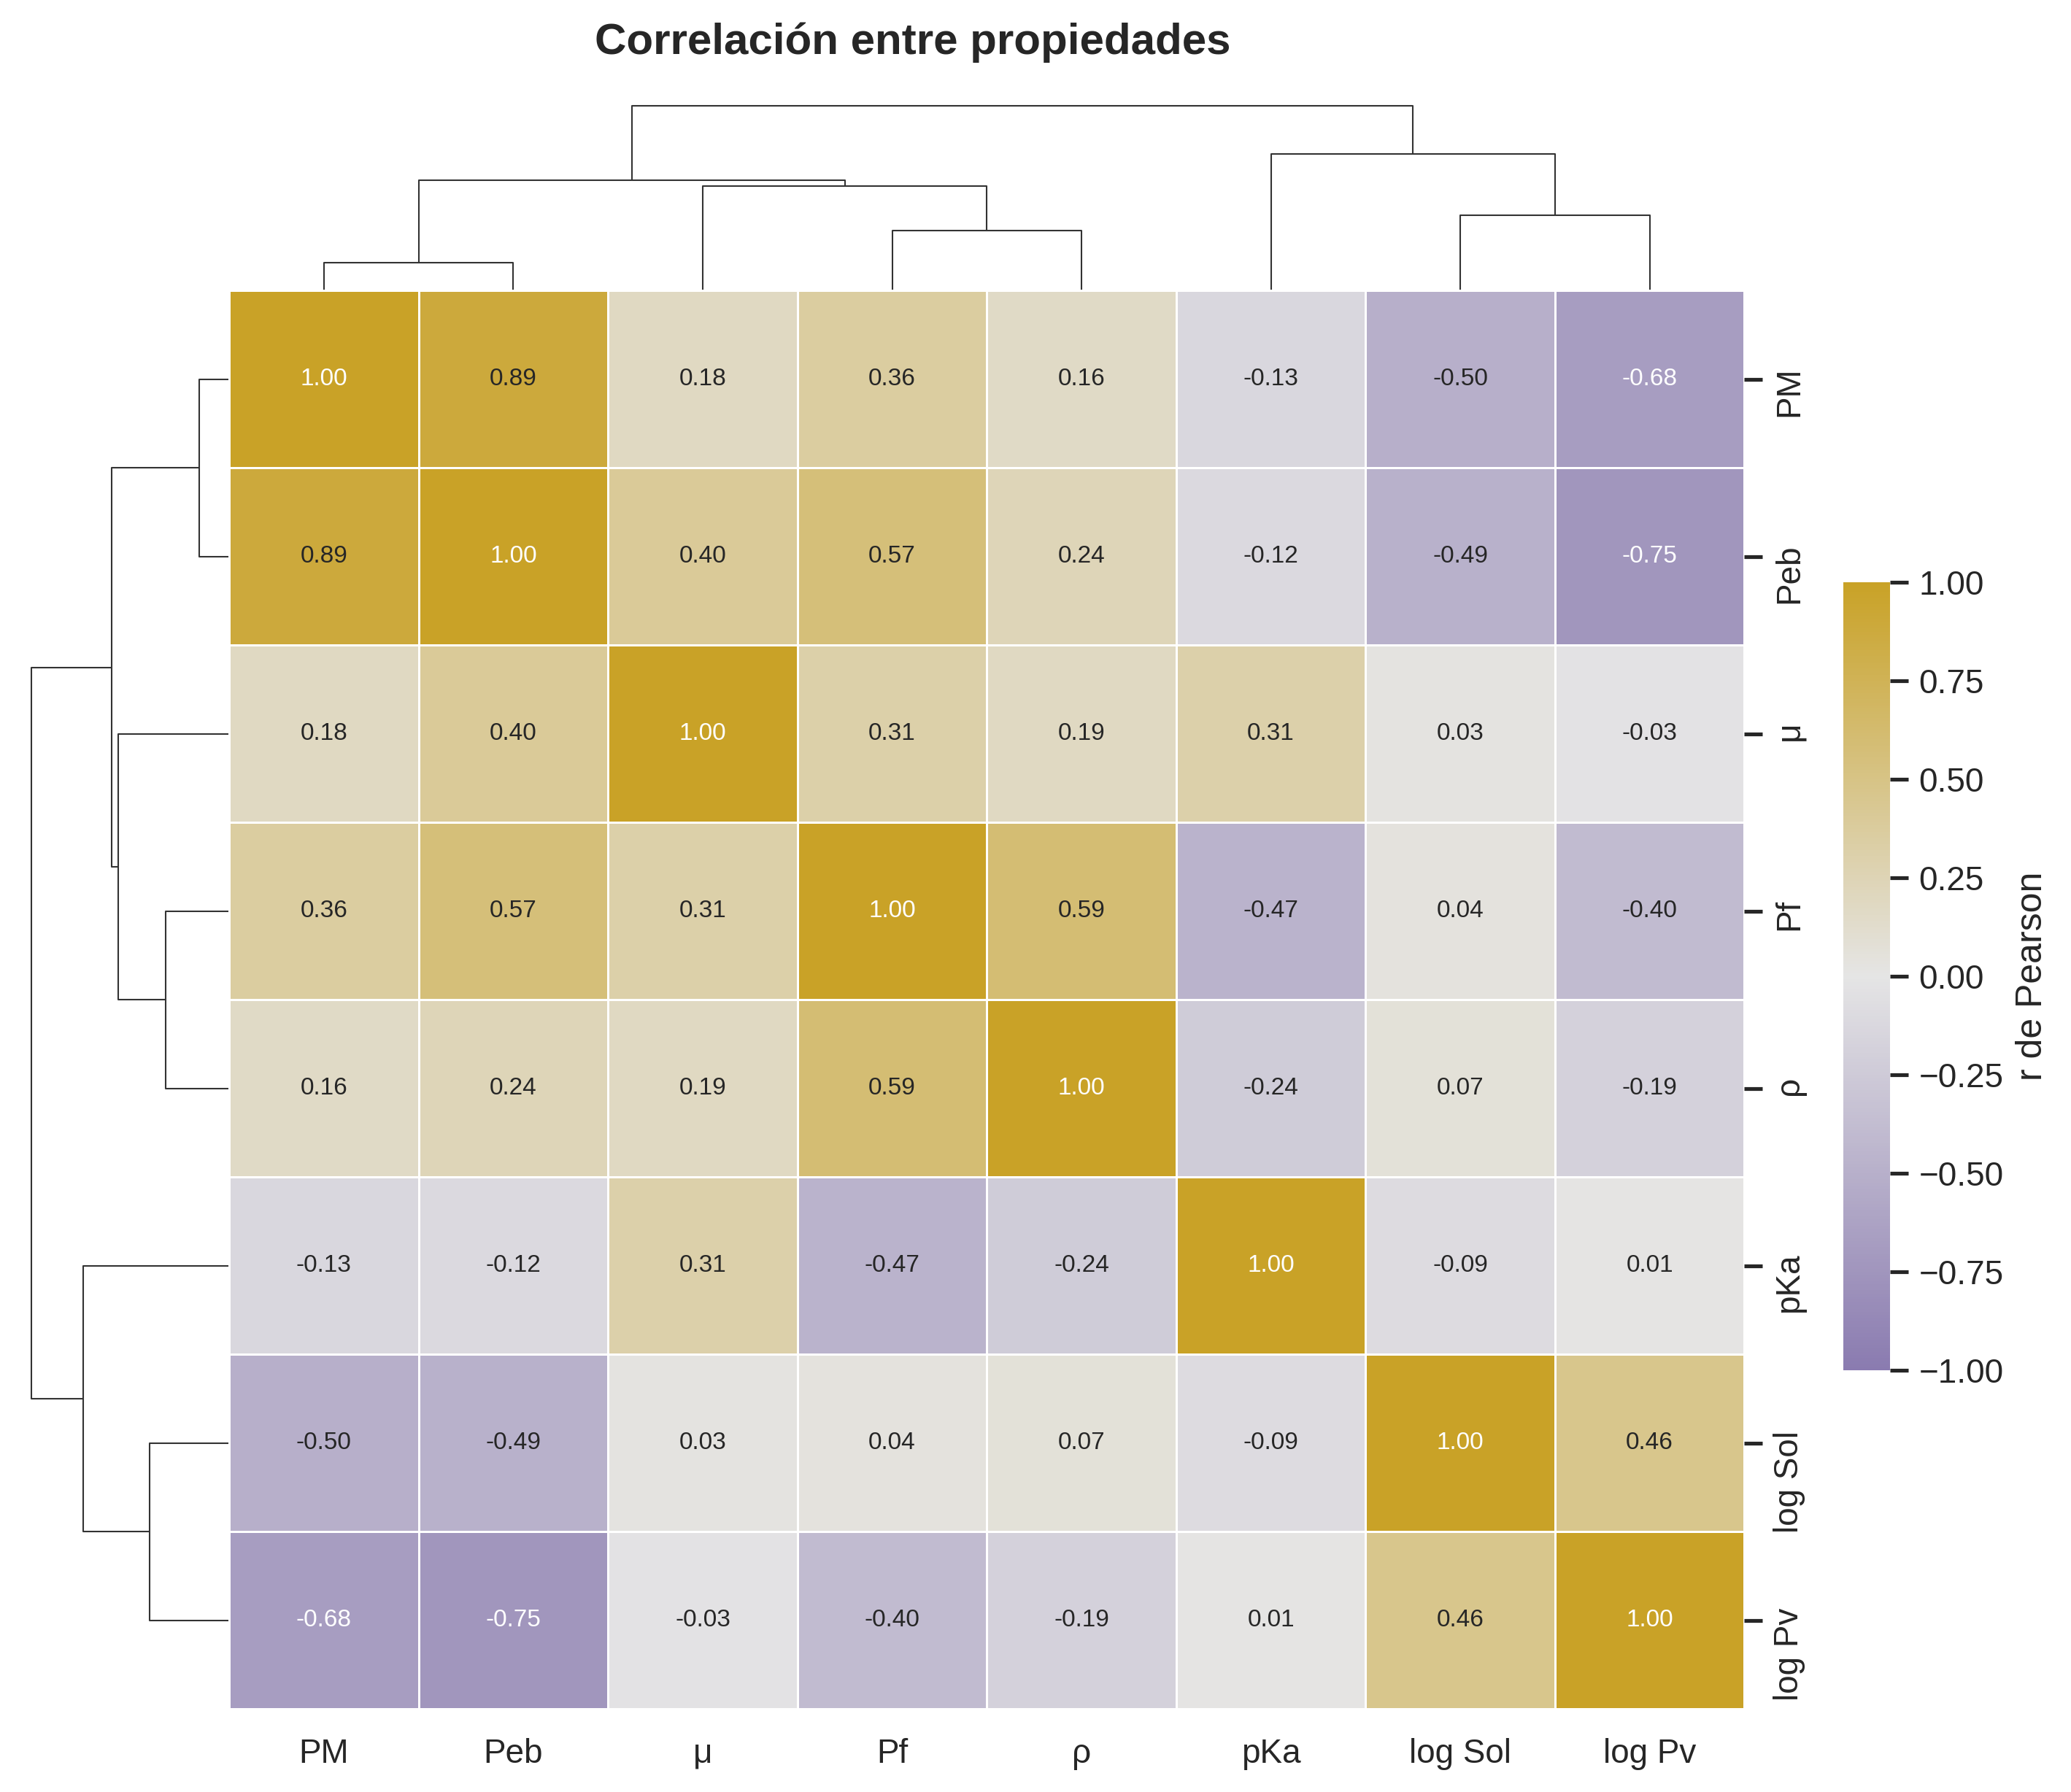
\includegraphics[width=\columnwidth]{01_mapa_correlacion.png}
\caption{Correlación de Pearson entre las propiedades de todos los compuestos del conjunto. El dendrograma agrupa las propiedades que se comportan de forma similar.}
\label{fig:correlacion}
\end{figure}

La Figura~\ref{fig:correlacion} muestra que la relación más fuerte es PM–Peb ($r$ = 0.89), seguida de Peb–log Pv ($-$0.75) y PM–log Pv ($-$0.68), debido a que las moléculas más grandes tienen más fuerzas intermoleculares, hierven a mayor temperatura y se evaporan menos. El dendrograma agrupa PM con Peb, Pf con $\rho$ y log Sol con log Pv.
\begin{figure*}[!t]
\centering
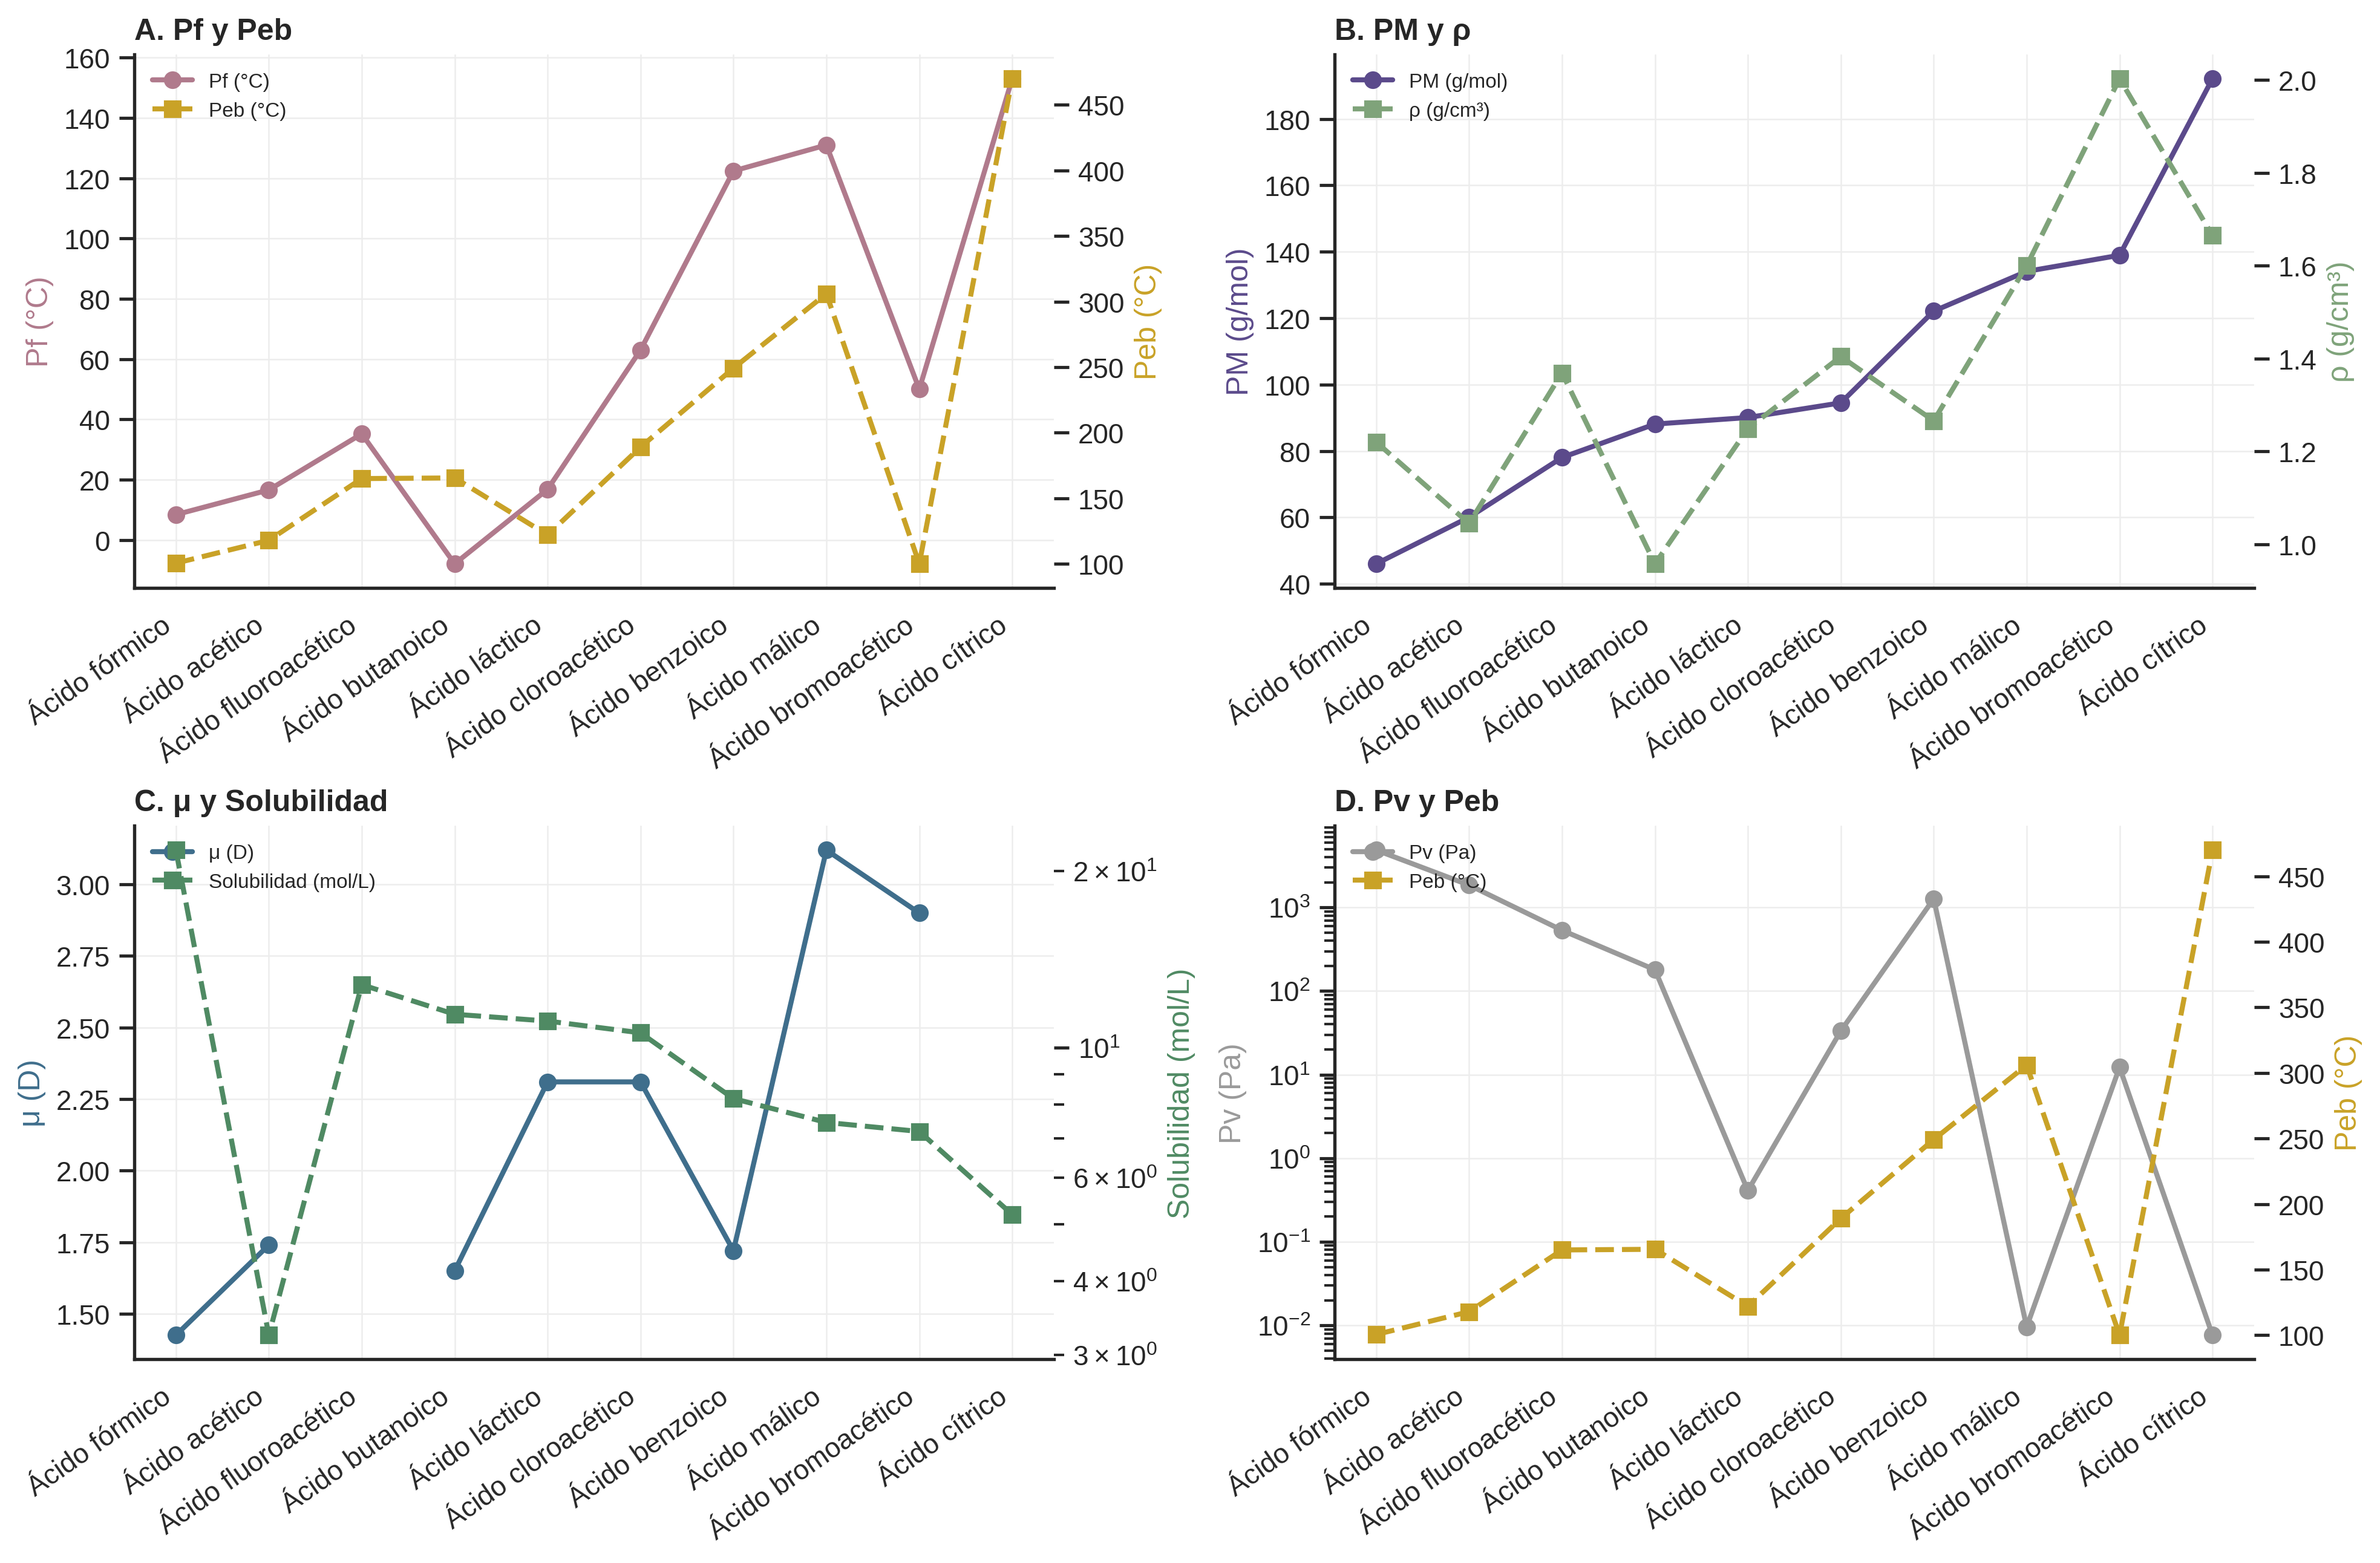
\includegraphics[width=0.9\textwidth]{04_doble_eje_propiedades.png}
\caption{Propiedades de los diez ácidos ordenados por peso molecular, en pares con doble eje: (A) Pf y Peb, (B) PM y densidad, (C) momento dipolar y solubilidad, (D) presión de vapor y Peb.}
\label{fig:dobleeje}
\end{figure*}

En la Figura~\ref{fig:dobleeje}, el Pf y el Peb aumentan con el PM (Spearman $\rho_s$ = 0.70, $p$ = 0.025), al igual que la densidad ($\rho_s$ = 0.82, $p$ = 0.004), que es mayor en los haloácidos por la masa del halógeno. Las parejas $\mu$–solubilidad ($\rho_s$ = $-$0.61, $p$ = 0.11) y Pv–Peb ($\rho_s$ = $-$0.50, $p$ = 0.14) también muestran tendencias, pero no son significativas porque la muestra ($N$ = 10) es pequeña.

\begin{figure*}[!t]
\centering
\begin{subfigure}[t]{0.49\textwidth}\centering
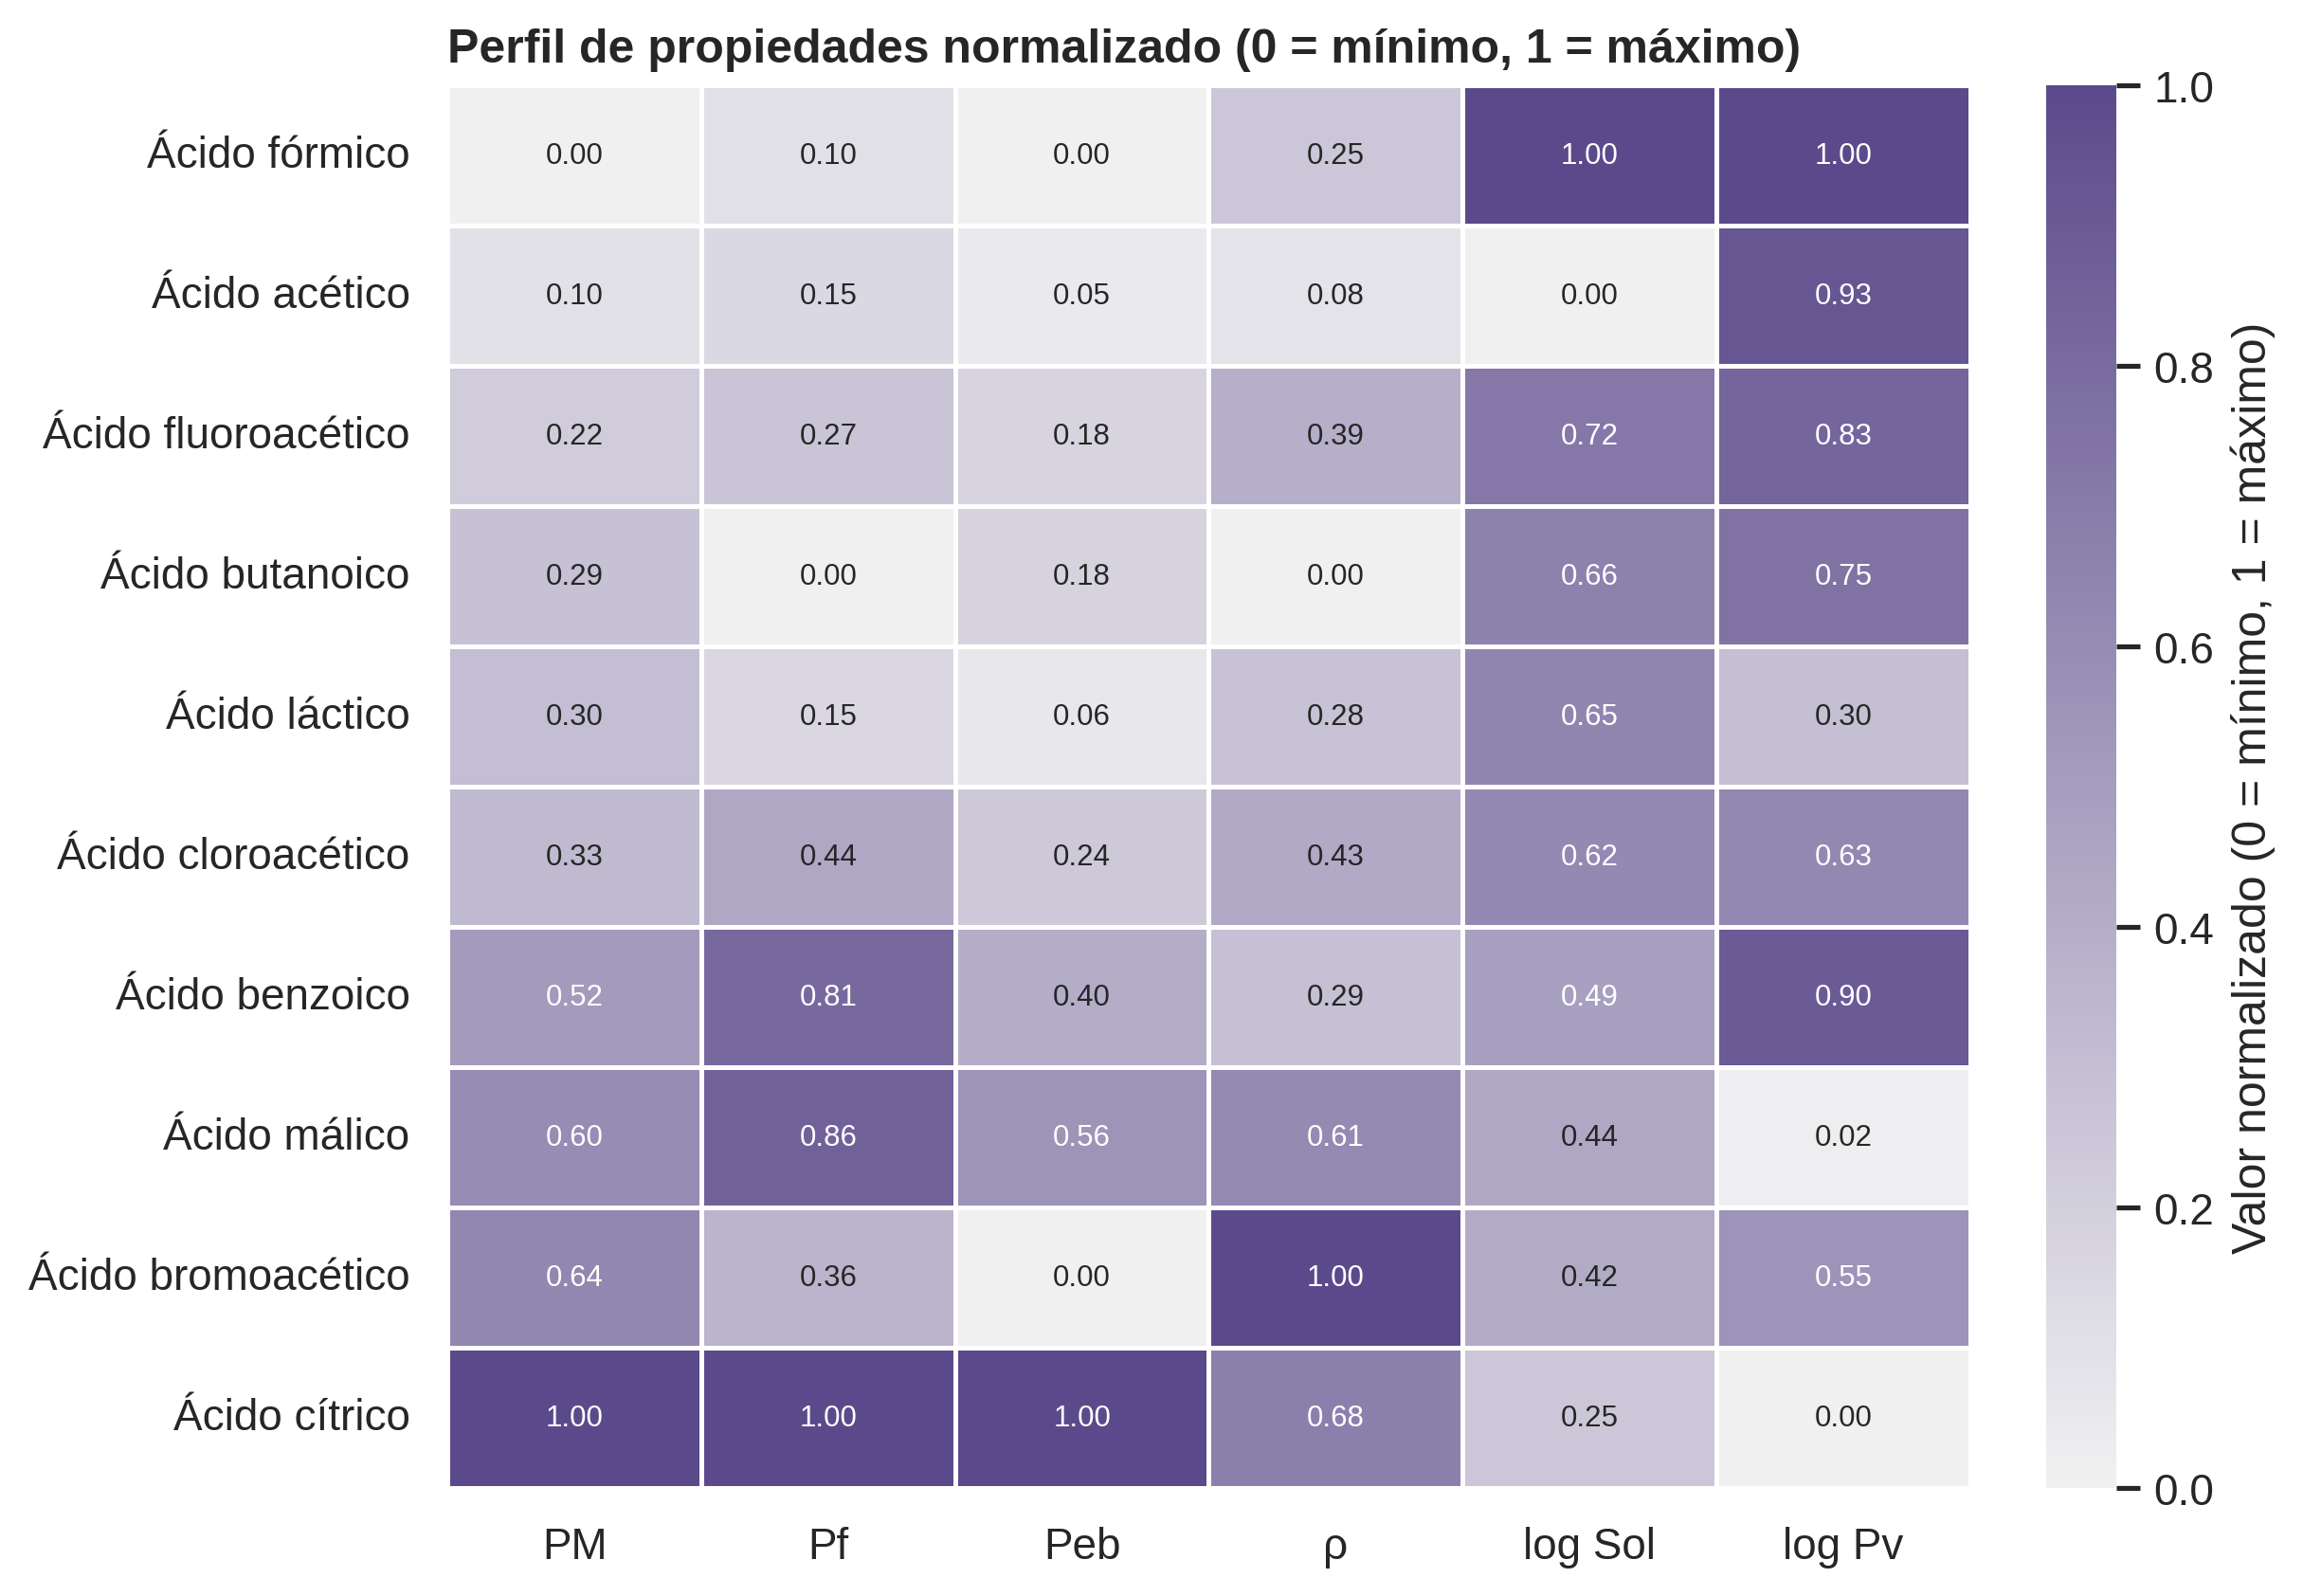
\includegraphics[width=\linewidth]{05_propiedades_normalizadas.png}
\caption{Propiedades normalizadas (0 = mínimo, 1 = máximo).}
\label{fig:normalizado}
\end{subfigure}\hfill
\begin{subfigure}[t]{0.49\textwidth}\centering
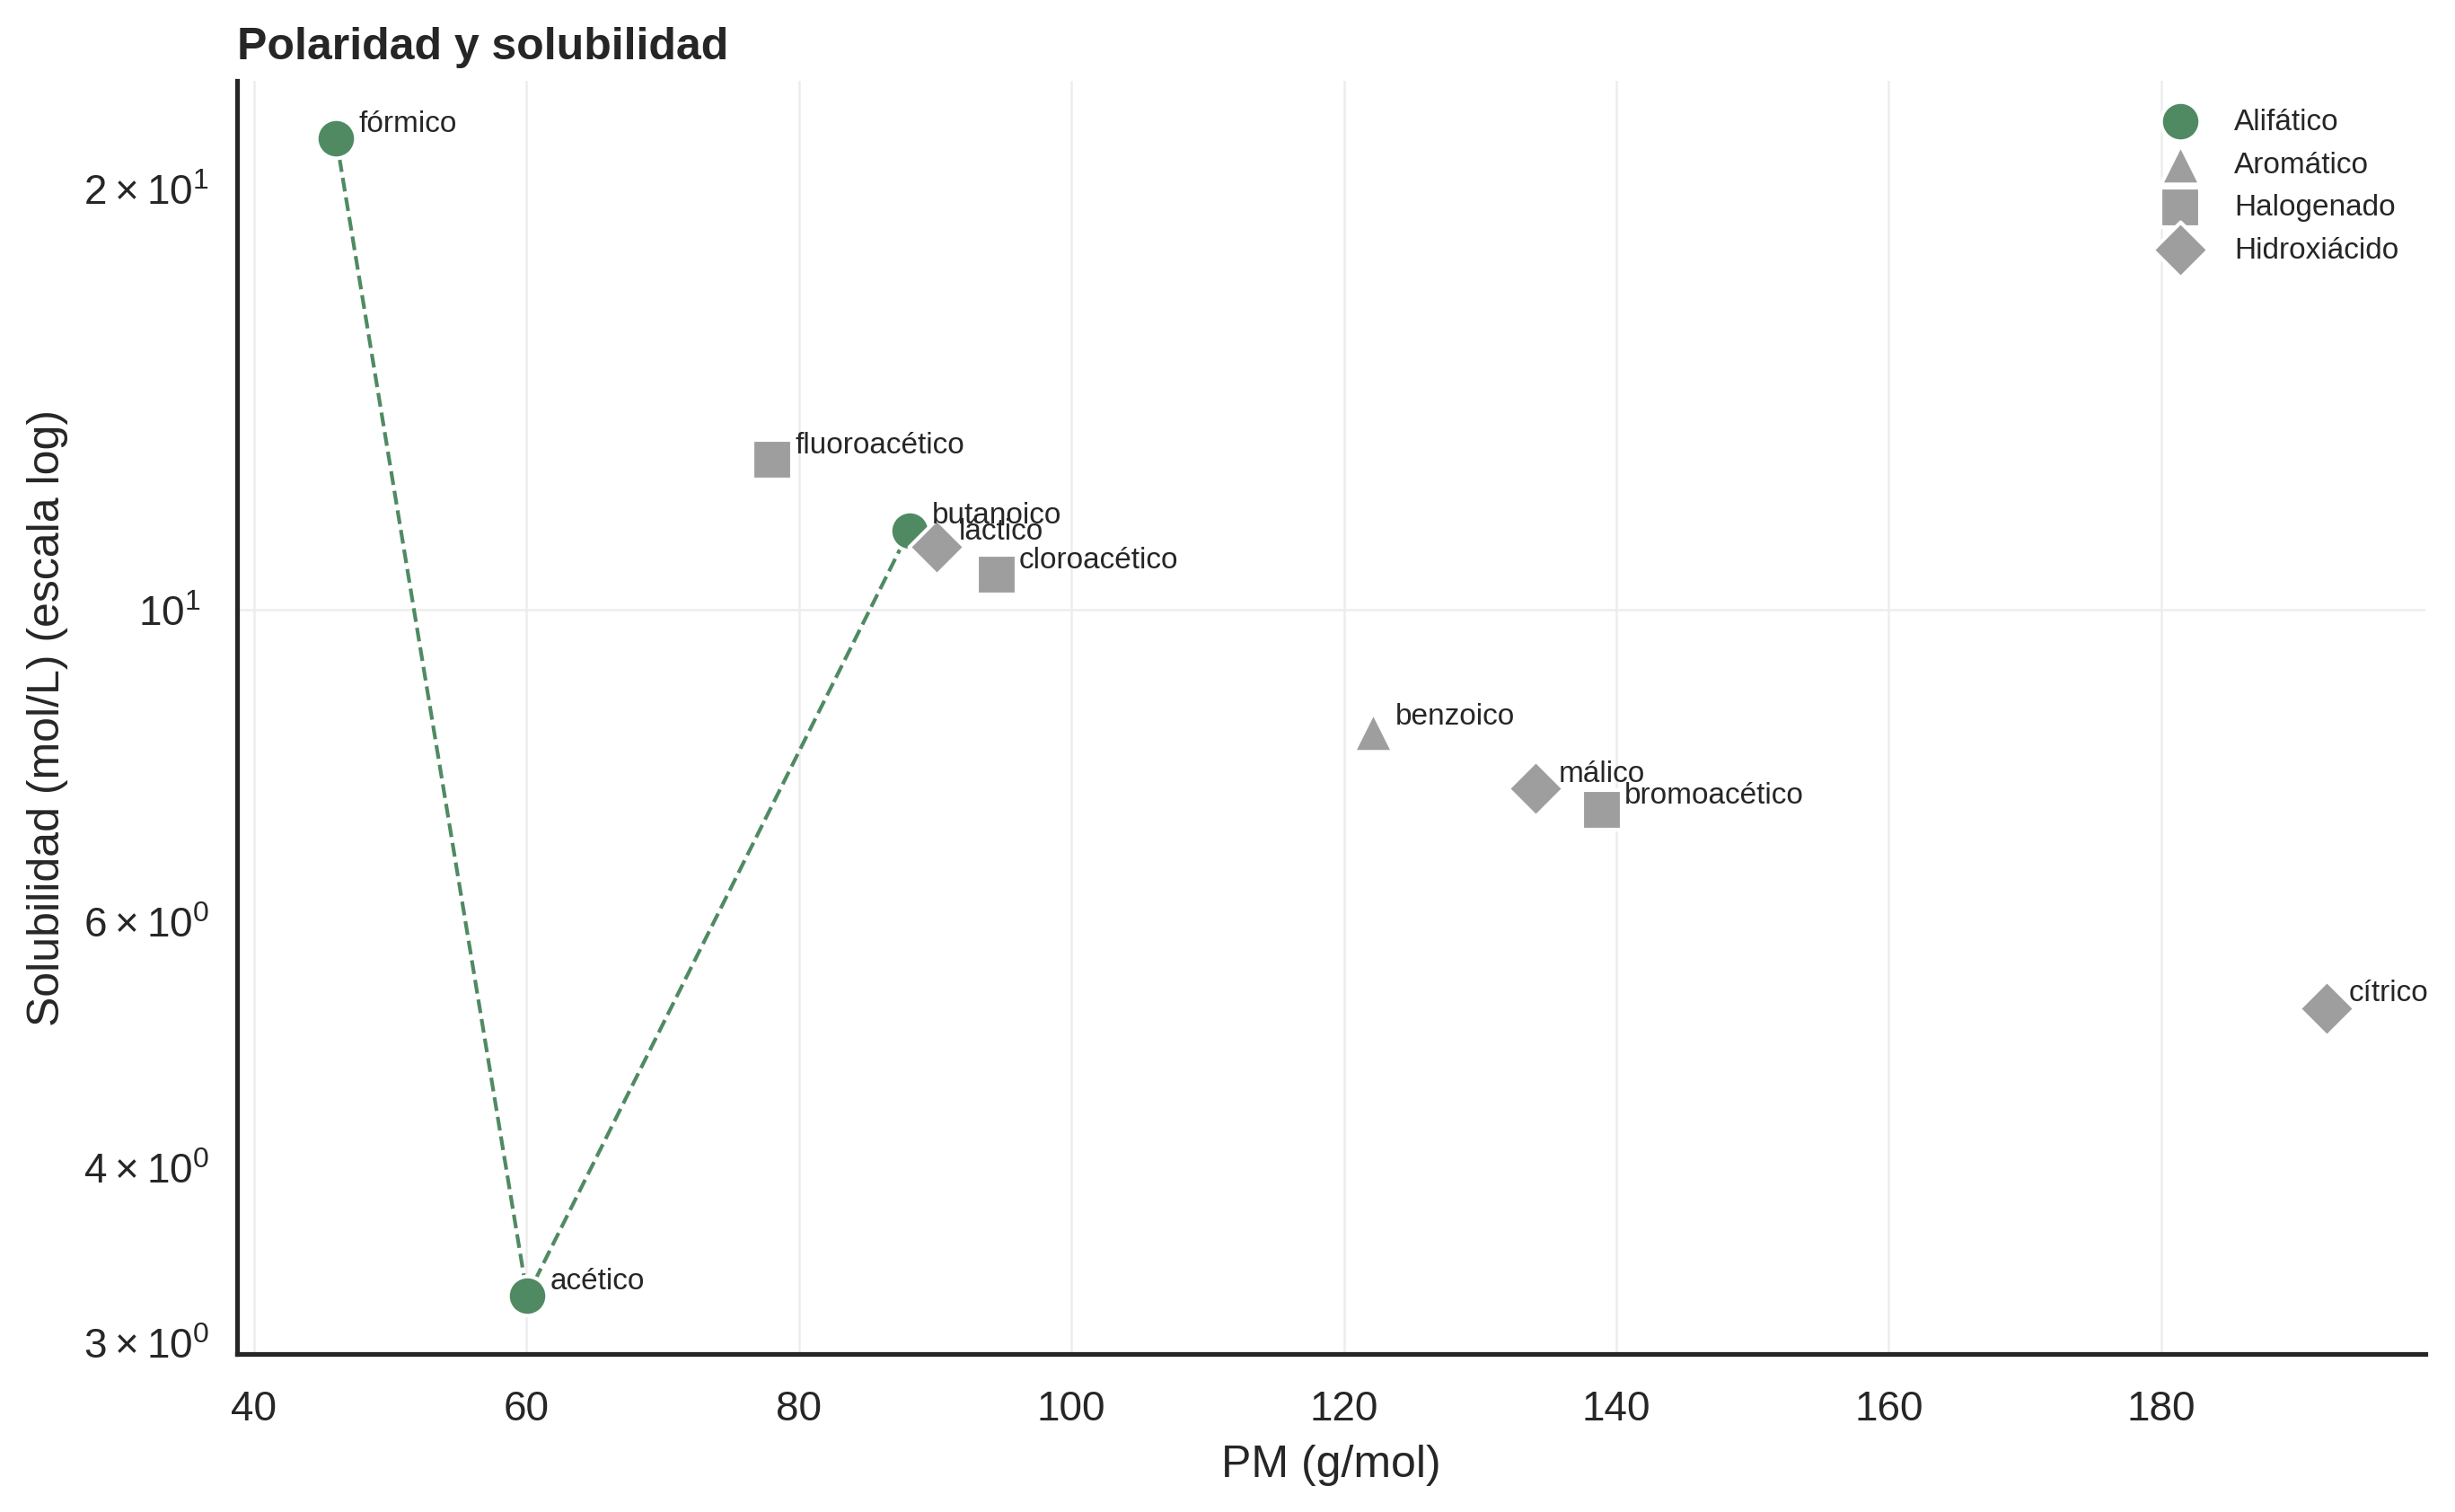
\includegraphics[width=\linewidth]{06_solubilidad_estructura.png}
\caption{Solubilidad en agua frente al peso molecular.}
\label{fig:solubilidad}
\end{subfigure}
\caption{Perfil de los diez ácidos. En (a) se excluyen el pKa (no se compara entre sustancias) y $\mu$ (falta en dos ácidos); en (b) el marcador indica el grupo estructural.}
\label{fig:perfil}
\end{figure*}

La Figura~\ref{fig:normalizado} resume el perfil de cada ácido en escala mínimo–máximo. En la serie alifática la solubilidad baja del ácido fórmico (21.7~mol/L) al butanoico, lo que concuerda con el aumento de la parte hidrocarbonada \cite{Schroeder2010}, mientras que los hidroxiácidos se mantienen solubles por sus grupos –OH adicionales (Figura~\ref{fig:solubilidad}). Con diez ácidos esta tendencia no es significativa ($\rho_s$ = $-$0.56, $p$ = 0.09).

\subsection{Tendencias en los productos y reactivos}

\begin{figure*}[!t]
\centering
\begin{subfigure}[t]{0.329\textwidth}\centering
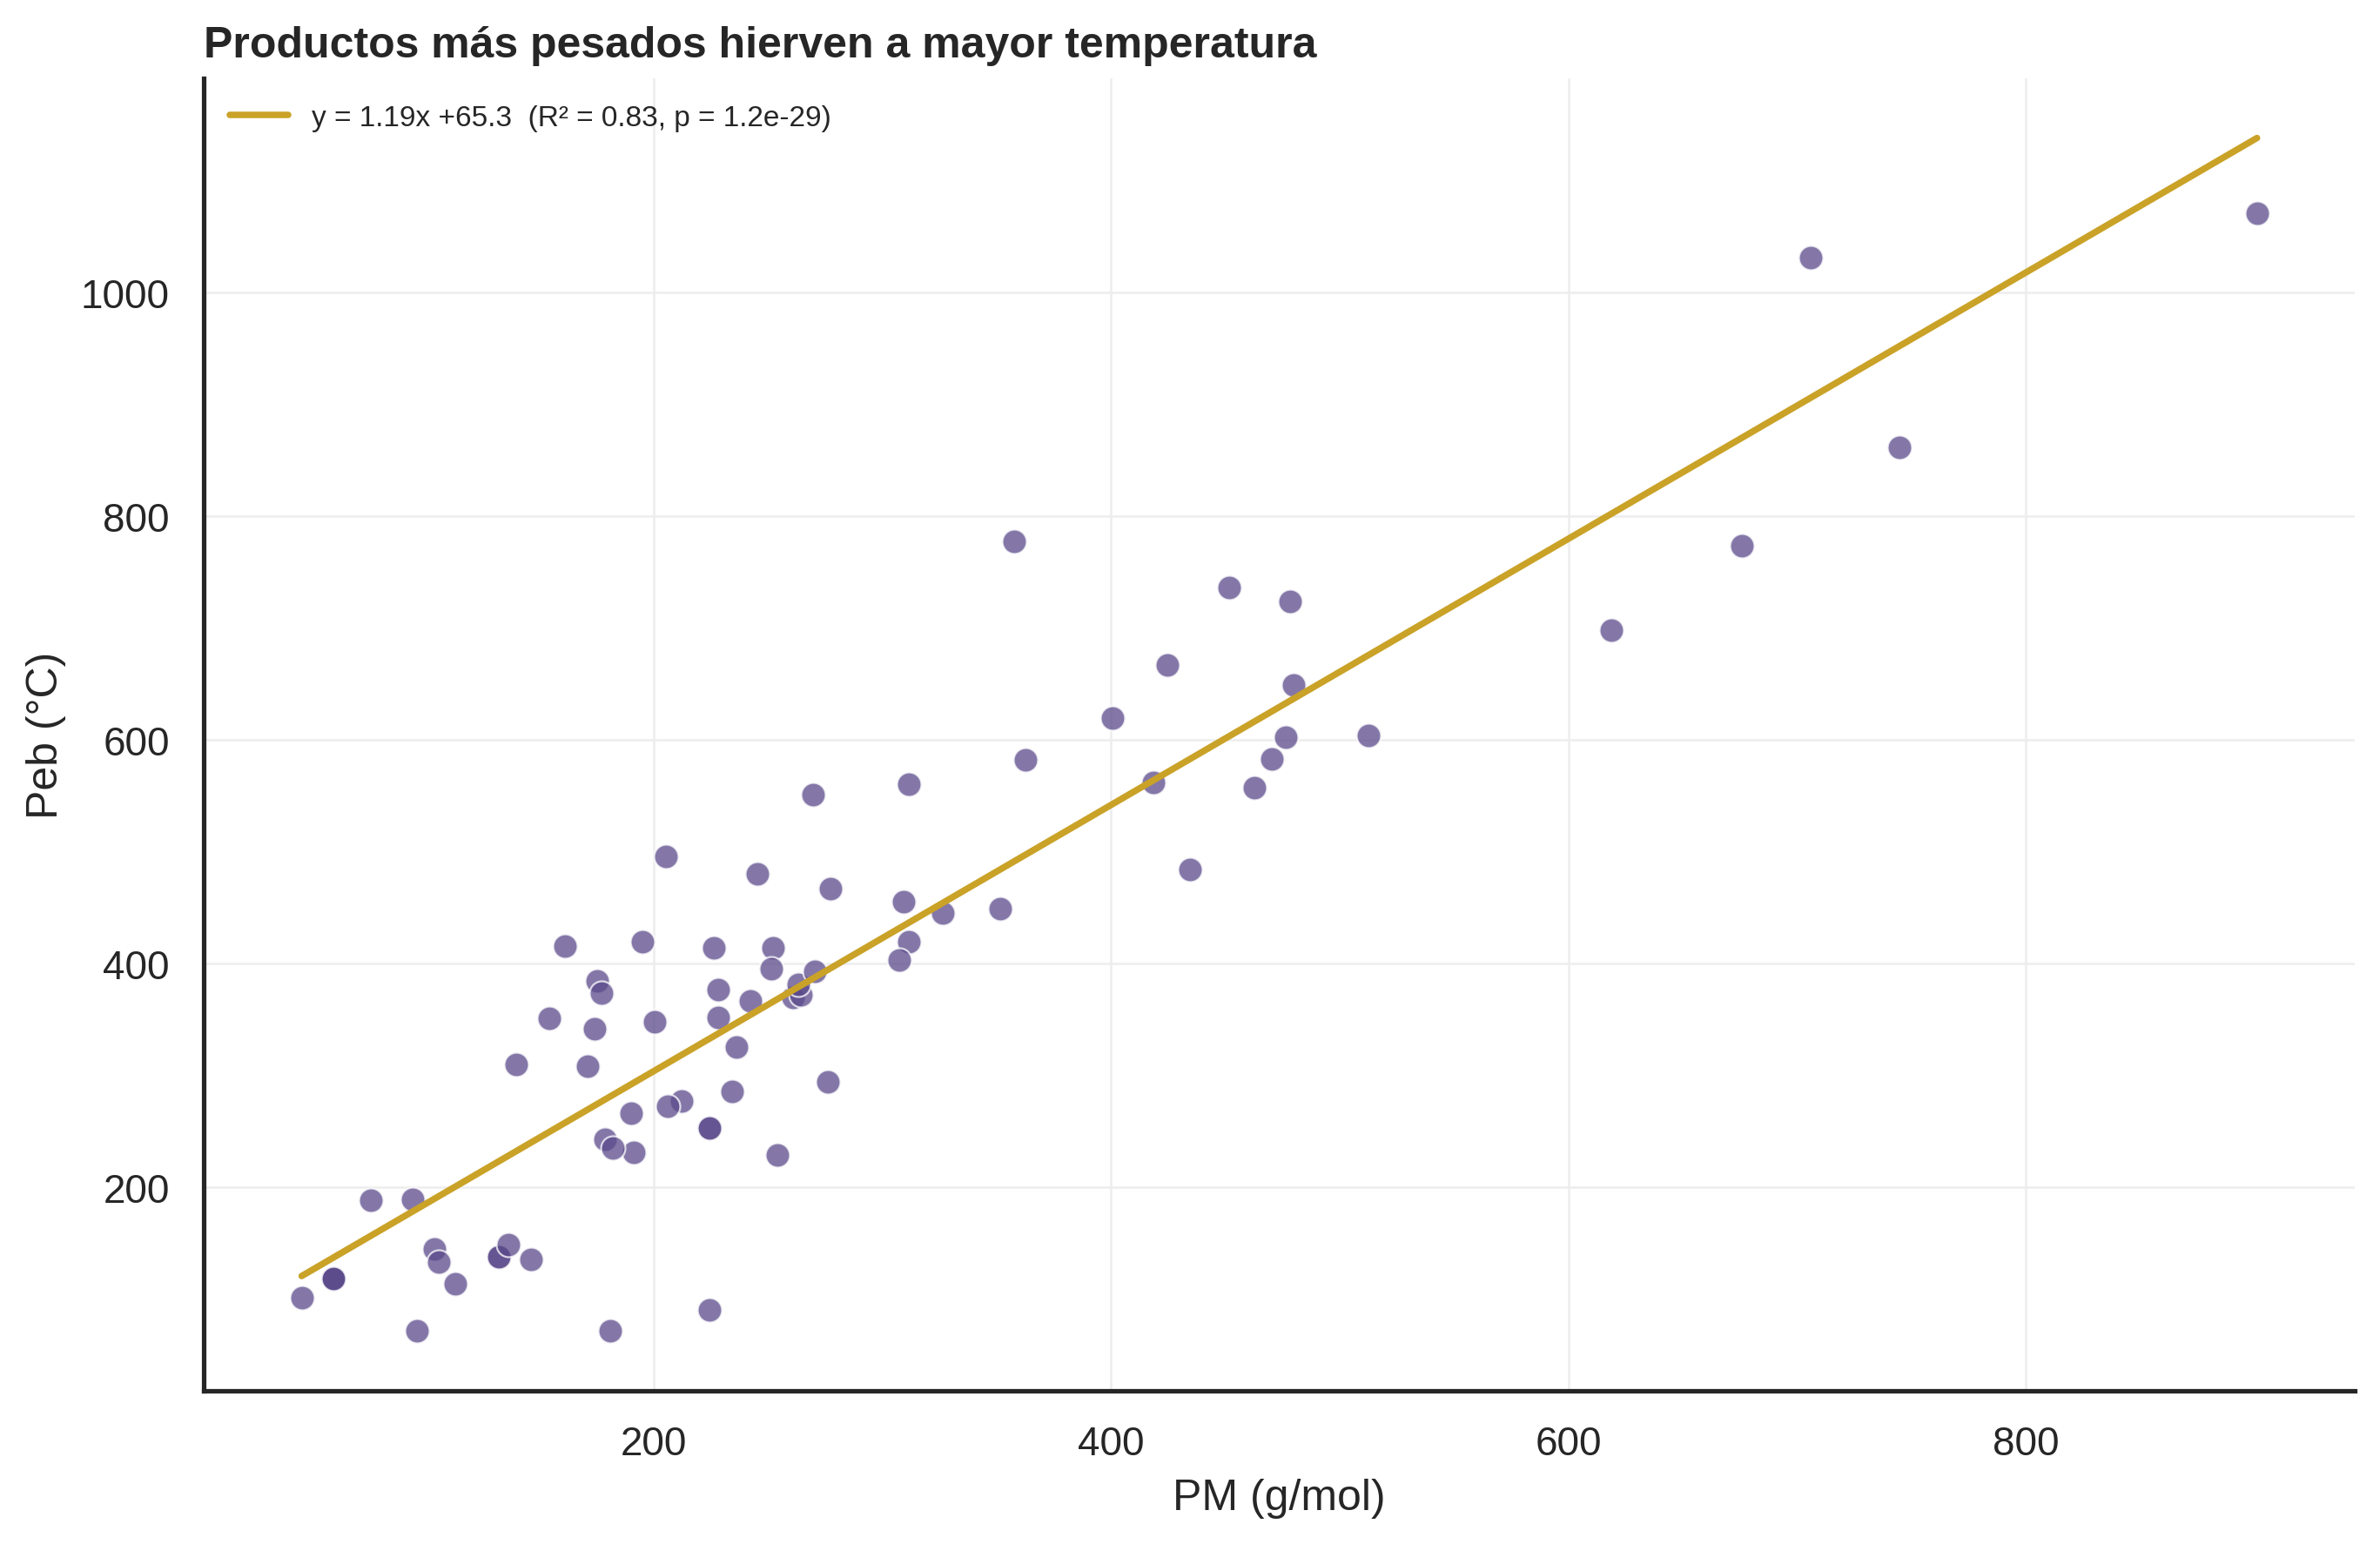
\includegraphics[width=\linewidth]{07_PM_vs_Peb.png}
\caption{PM frente a Peb (productos).}
\label{fig:pmpeb}
\end{subfigure}\hfill
\begin{subfigure}[t]{0.329\textwidth}\centering
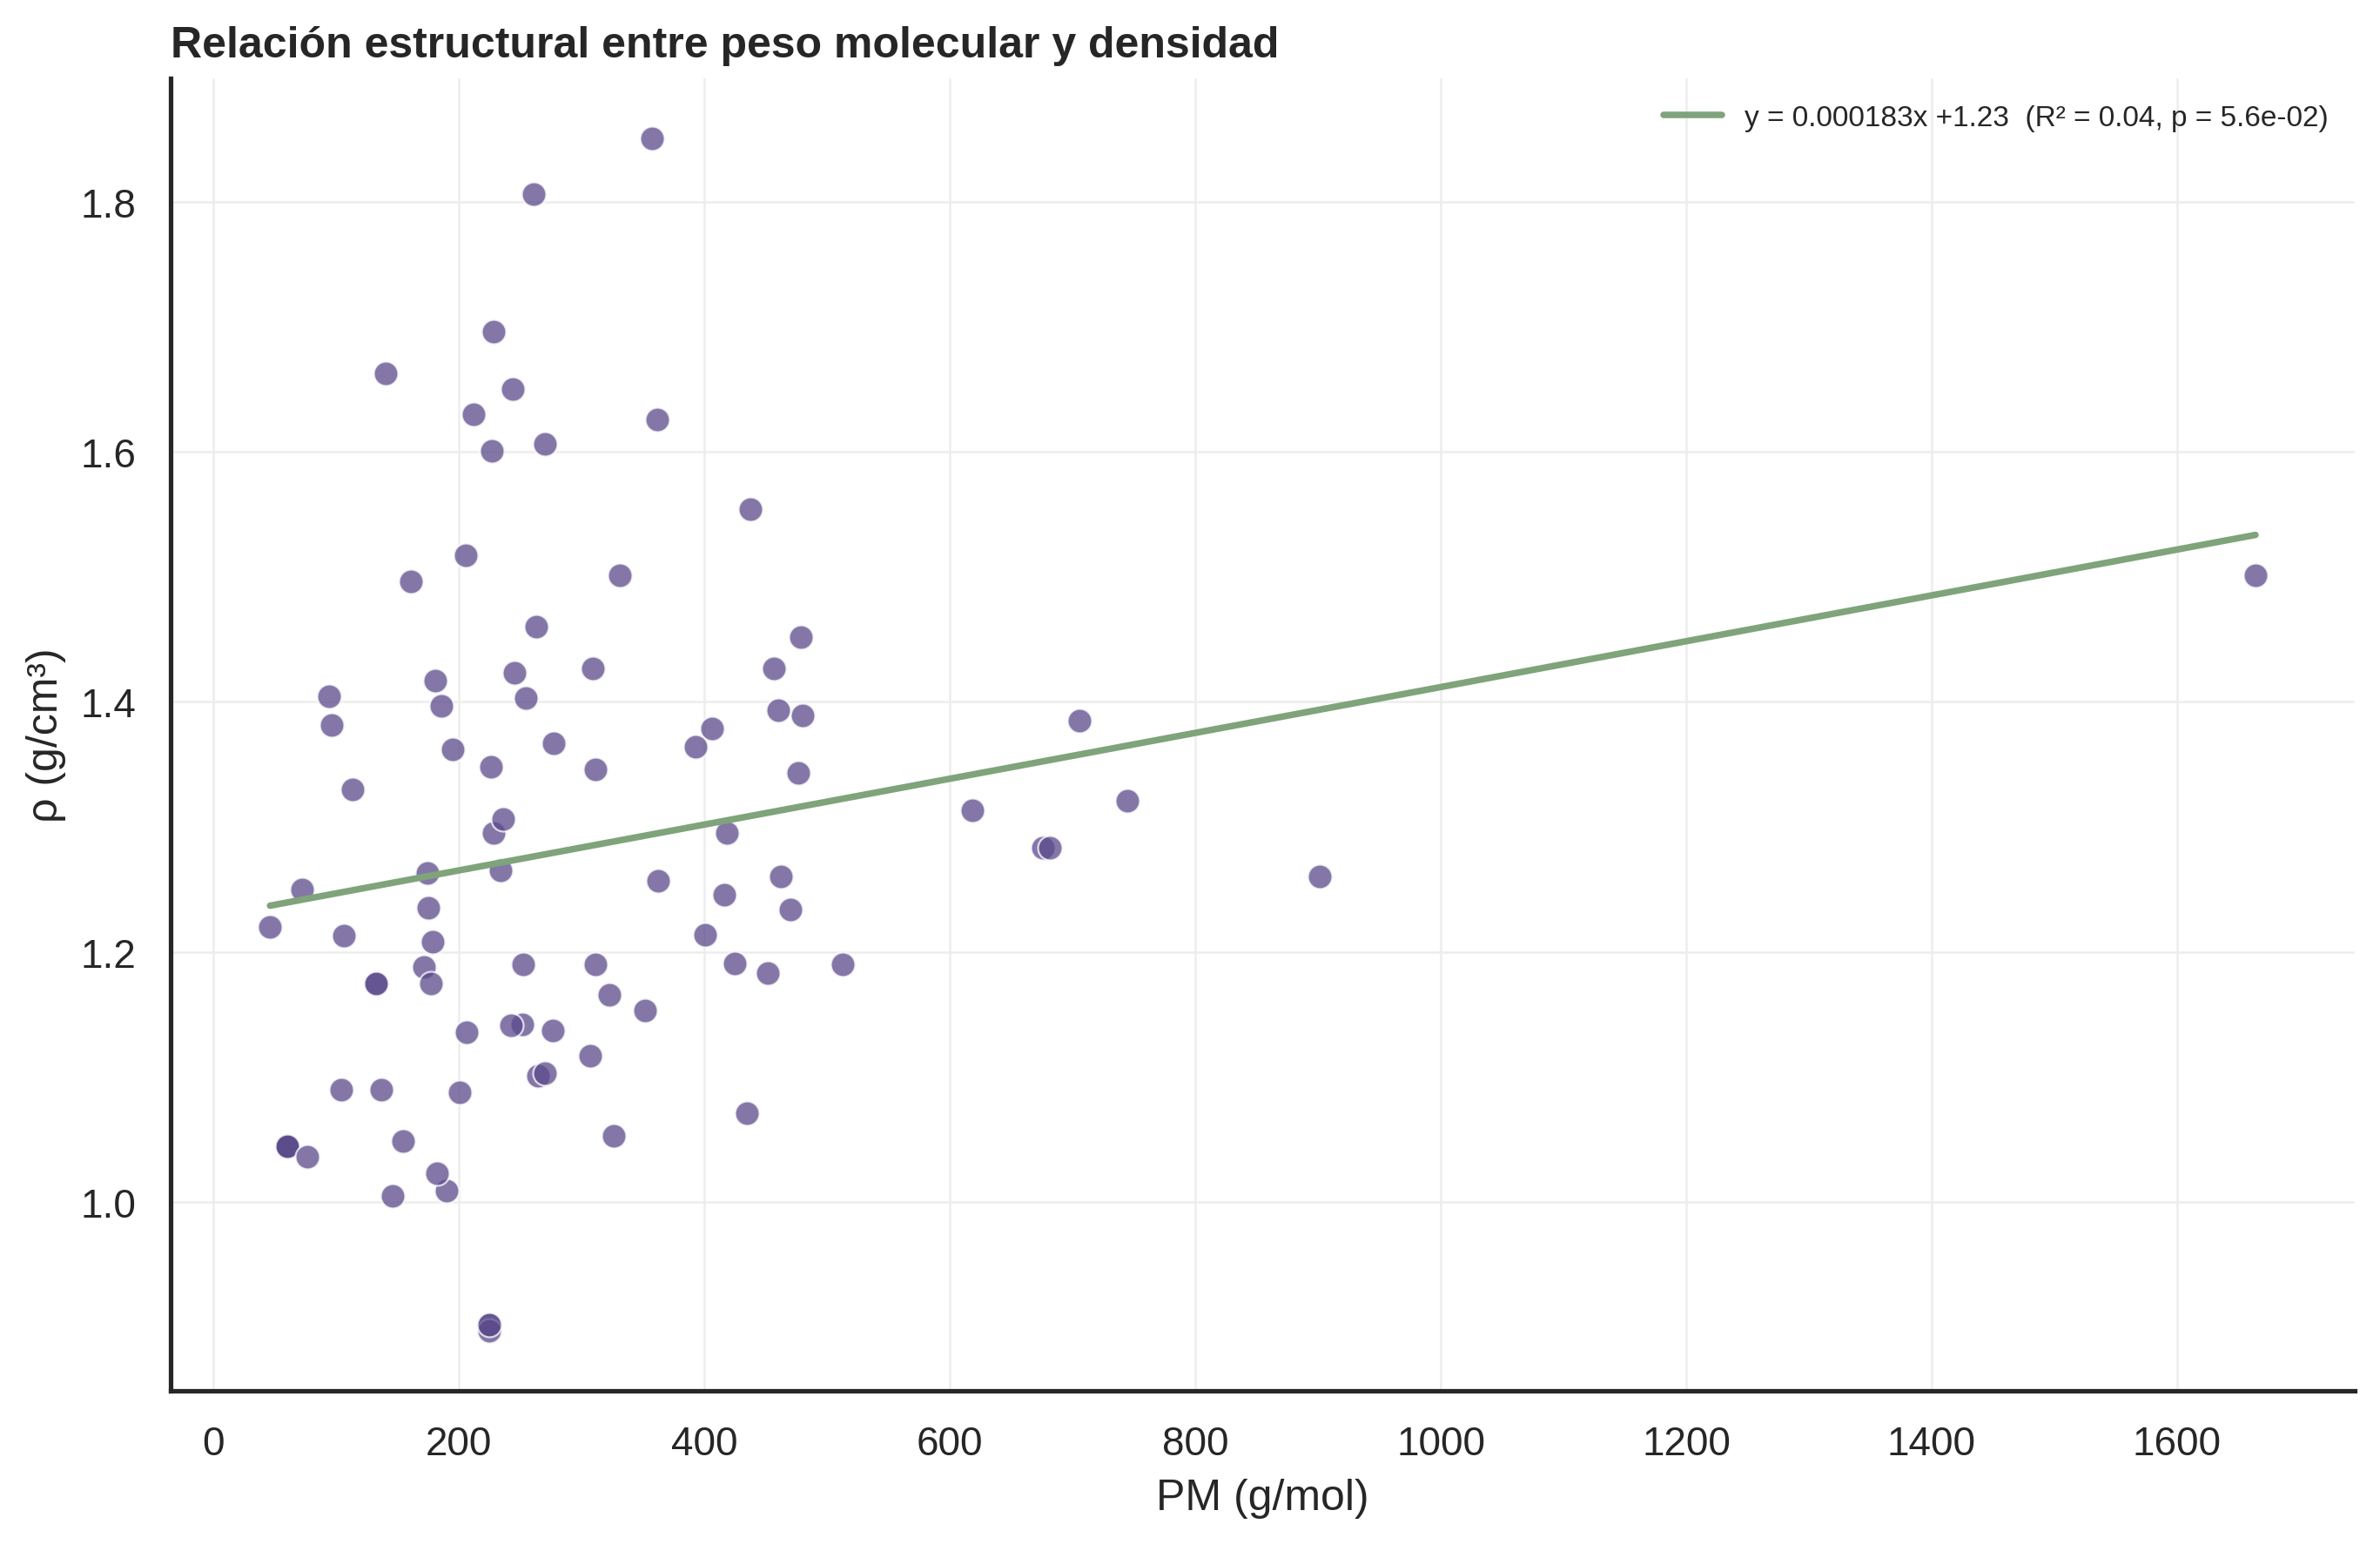
\includegraphics[width=\linewidth]{08_PM_vs_densidad.png}
\caption{PM frente a densidad (productos).}
\label{fig:pmrho}
\end{subfigure}\hfill
\begin{subfigure}[t]{0.329\textwidth}\centering
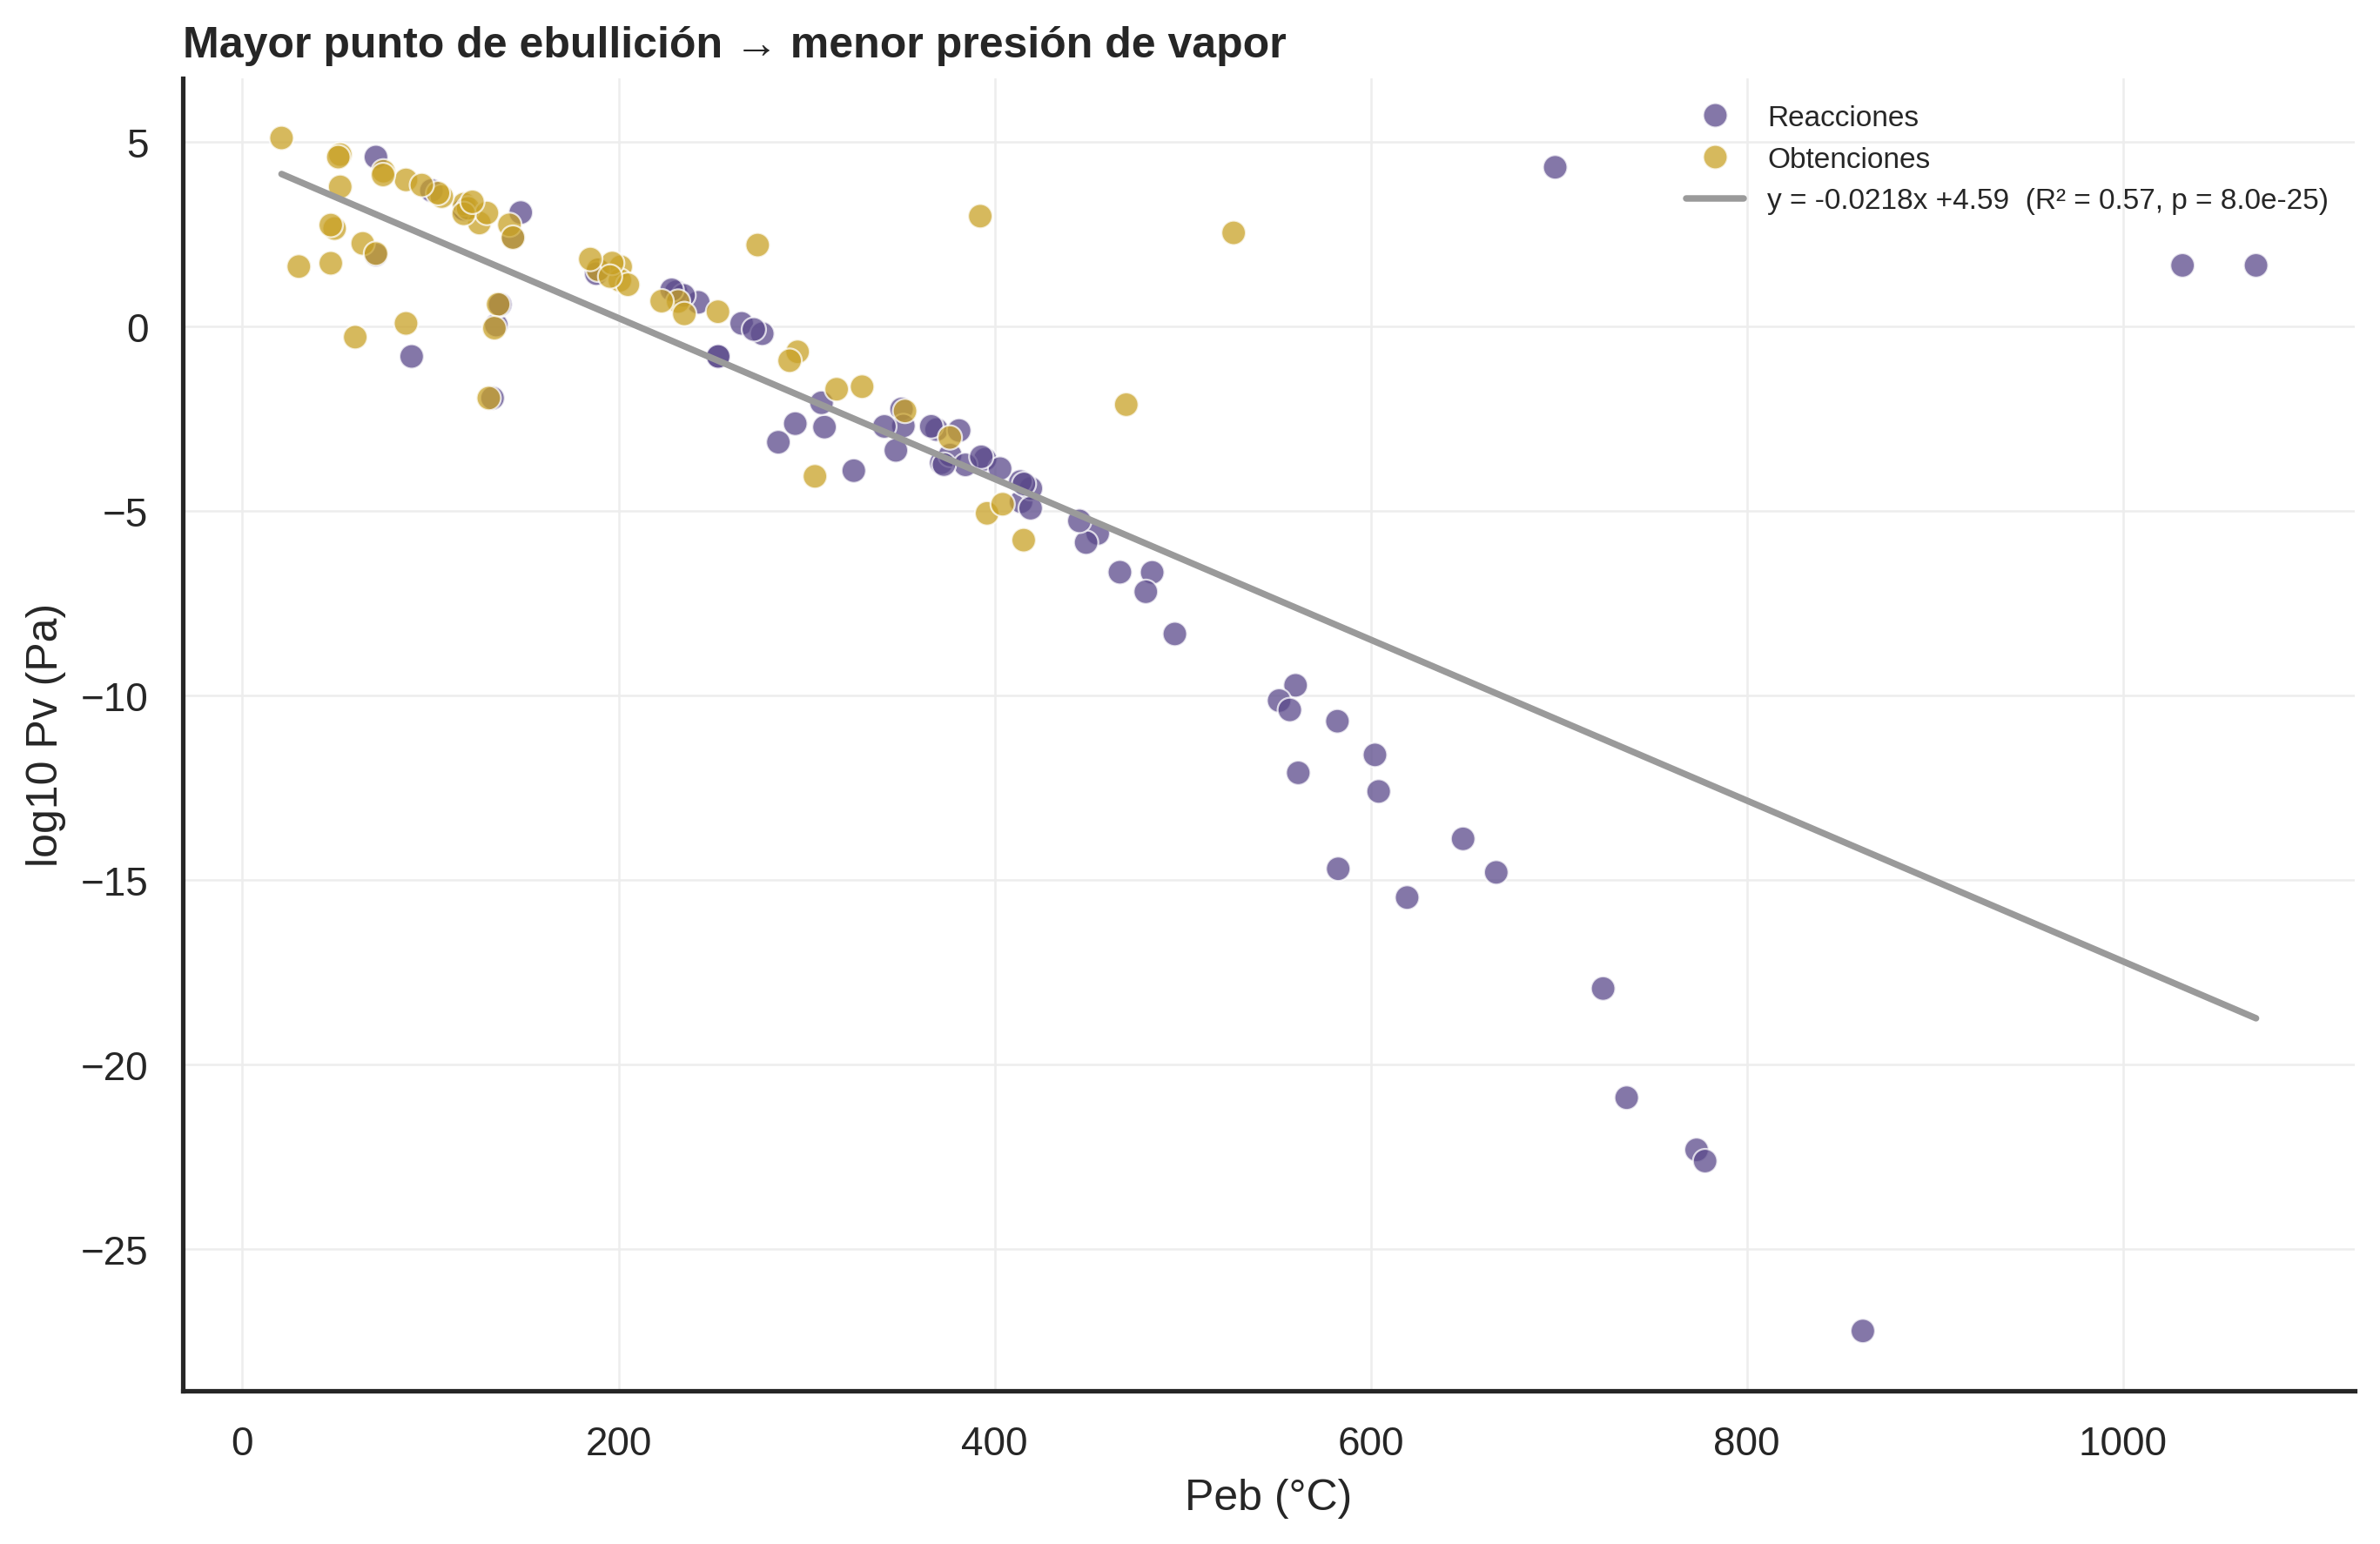
\includegraphics[width=\linewidth]{09_Peb_vs_Pv.png}
\caption{Peb frente a log Pv (productos y reactivos).}
\label{fig:pebpv}
\end{subfigure}
\caption{Relaciones entre propiedades de los compuestos de las reacciones, con su recta de regresión lineal.}
\label{fig:regresiones}
\end{figure*}

En los productos de las reacciones, el Peb crece con el PM: Peb = 1.19·PM + 65 ($R^2$ = 0.83, $p$ = 1$\times$10$^{-29}$, $n$ = 75; Figura~\ref{fig:pmpeb}). El PM explica el 83\,\% de la variación del Peb, de acuerdo con el aumento de las fuerzas de London y, en los derivados con –OH o –NH, de los puentes de hidrógeno. En cambio, el PM casi no explica la densidad ($R^2$ = 0.04, $p$ = 0.056; Figura~\ref{fig:pmrho}), porque la densidad depende más de los heteroátomos (O, N, halógenos) que del tamaño.

La presión de vapor disminuye con el Peb (log Pv = $-$0.022·Peb + 4.59; $R^2$ = 0.57; Pearson $-$0.75, Spearman $-$0.81; $n$ = 128; Figura~\ref{fig:pebpv}). Ambas propiedades dependen de la energía necesaria para separar las moléculas; la relación es menos lineal que en compuestos sin grupos ácidos, lo que es coherente con la formación de dímeros por puente de hidrógeno \cite{Emelyanenko2020}. Tres productos con Peb entre 700 y 1070~\textdegree C presentan presiones de vapor altas que no son coherentes con su punto de ebullición.

\begin{figure*}[!t]
\centering
\begin{subfigure}[t]{0.49\textwidth}\centering
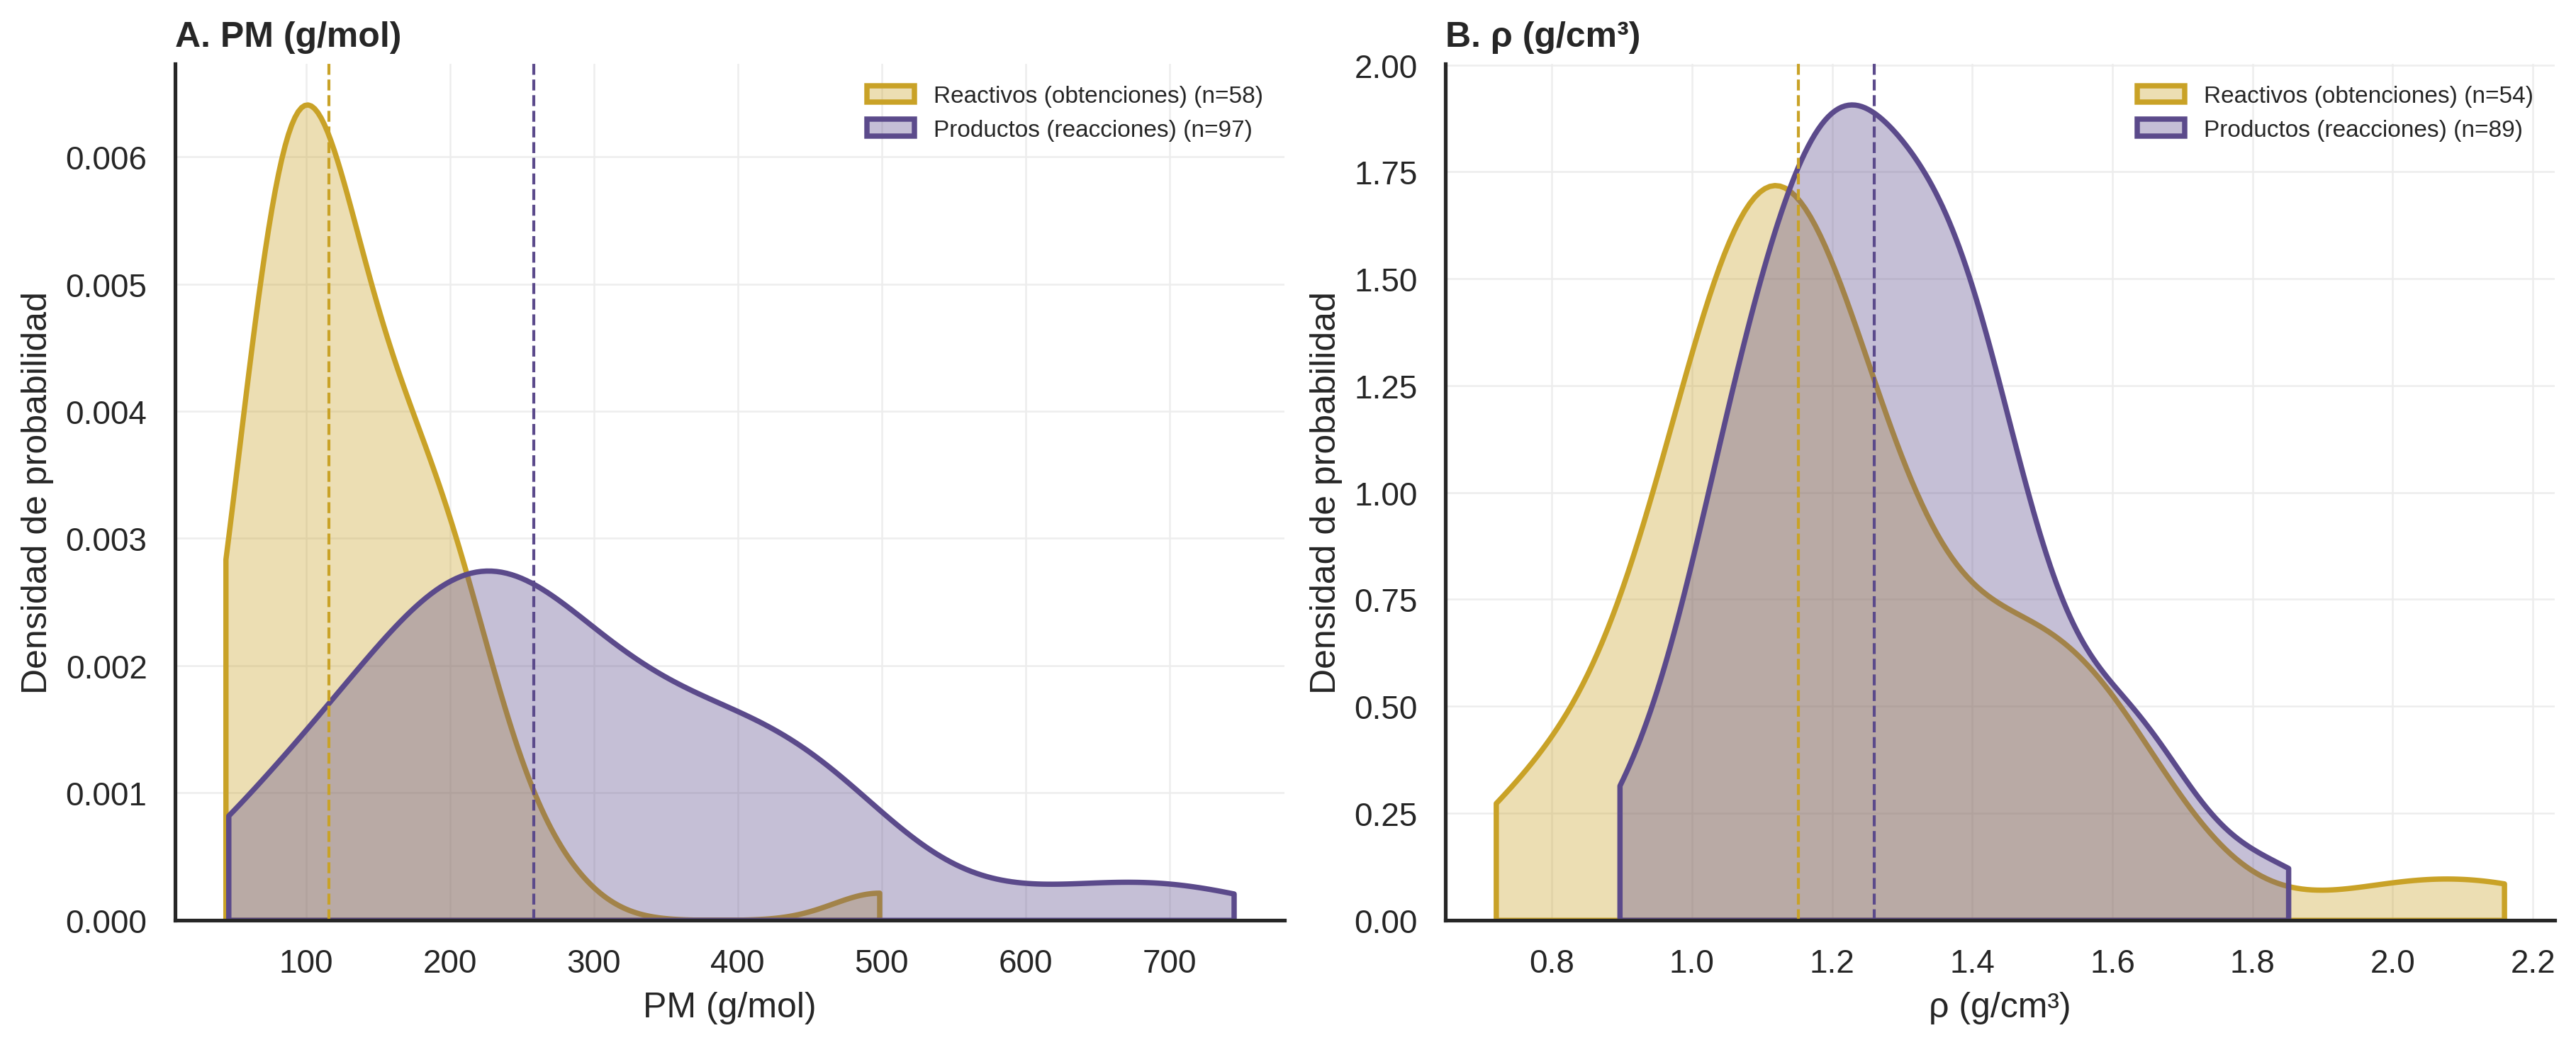
\includegraphics[width=\linewidth]{10_reactivos_vs_productos.png}
\caption{Densidad de probabilidad del PM (A) y de la densidad (B).}
\label{fig:kde}
\end{subfigure}\hfill
\begin{subfigure}[t]{0.49\textwidth}\centering
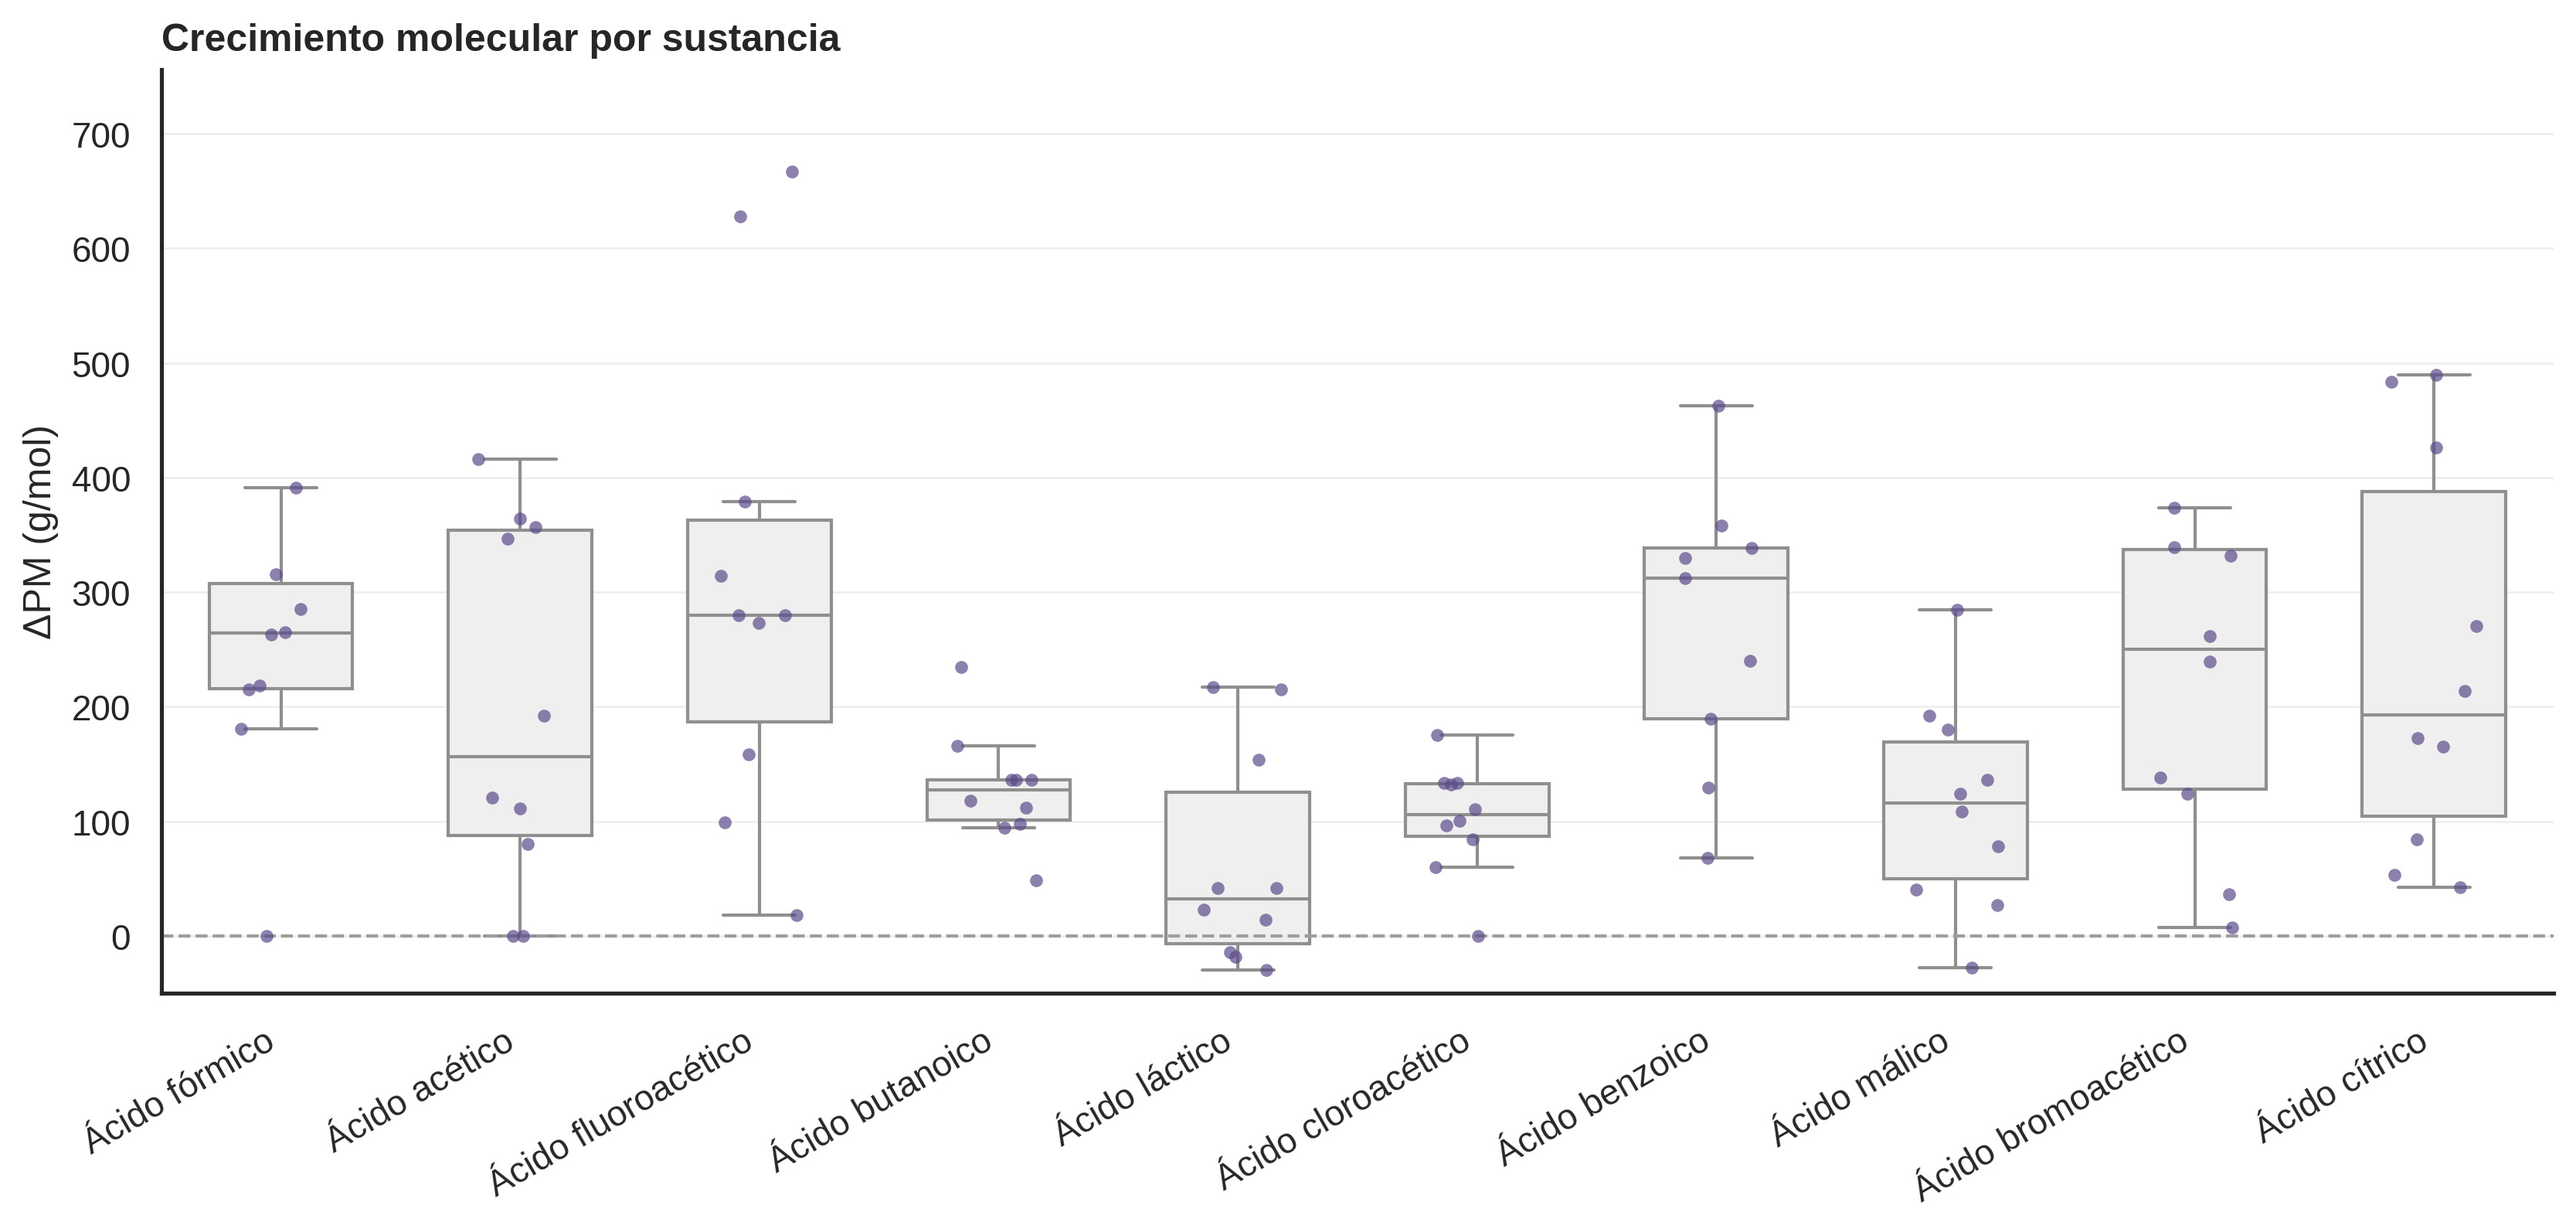
\includegraphics[width=\linewidth]{11_cambio_peso_molecular.png}
\caption{Cambio de peso molecular ($\Delta$PM) por ácido.}
\label{fig:dpm}
\end{subfigure}
\caption{Comparación de tamaño entre reactivos y productos. En (a) las líneas punteadas indican la mediana; en (b) $\Delta$PM = PM del producto $-$ PM del ácido.}
\label{fig:tamano}
\end{figure*}

Los productos son más pesados que los reactivos usados para obtener los ácidos (mediana 261 frente a 116~g/mol; Mann-Whitney $p$ = 1$\times$10$^{-12}$; Figura~\ref{fig:kde}), mientras que la diferencia de densidad no es significativa ($p$ = 0.065). En el 91\,\% de las reacciones el producto pesa más que el ácido de partida (Figura~\ref{fig:dpm}), con medianas de +313~g/mol en el benzoico y +33~g/mol en el láctico.

\subsection{Tipos de reacción y medio}

\begin{figure*}[!t]
\centering
\begin{subfigure}[t]{0.56\textwidth}\centering
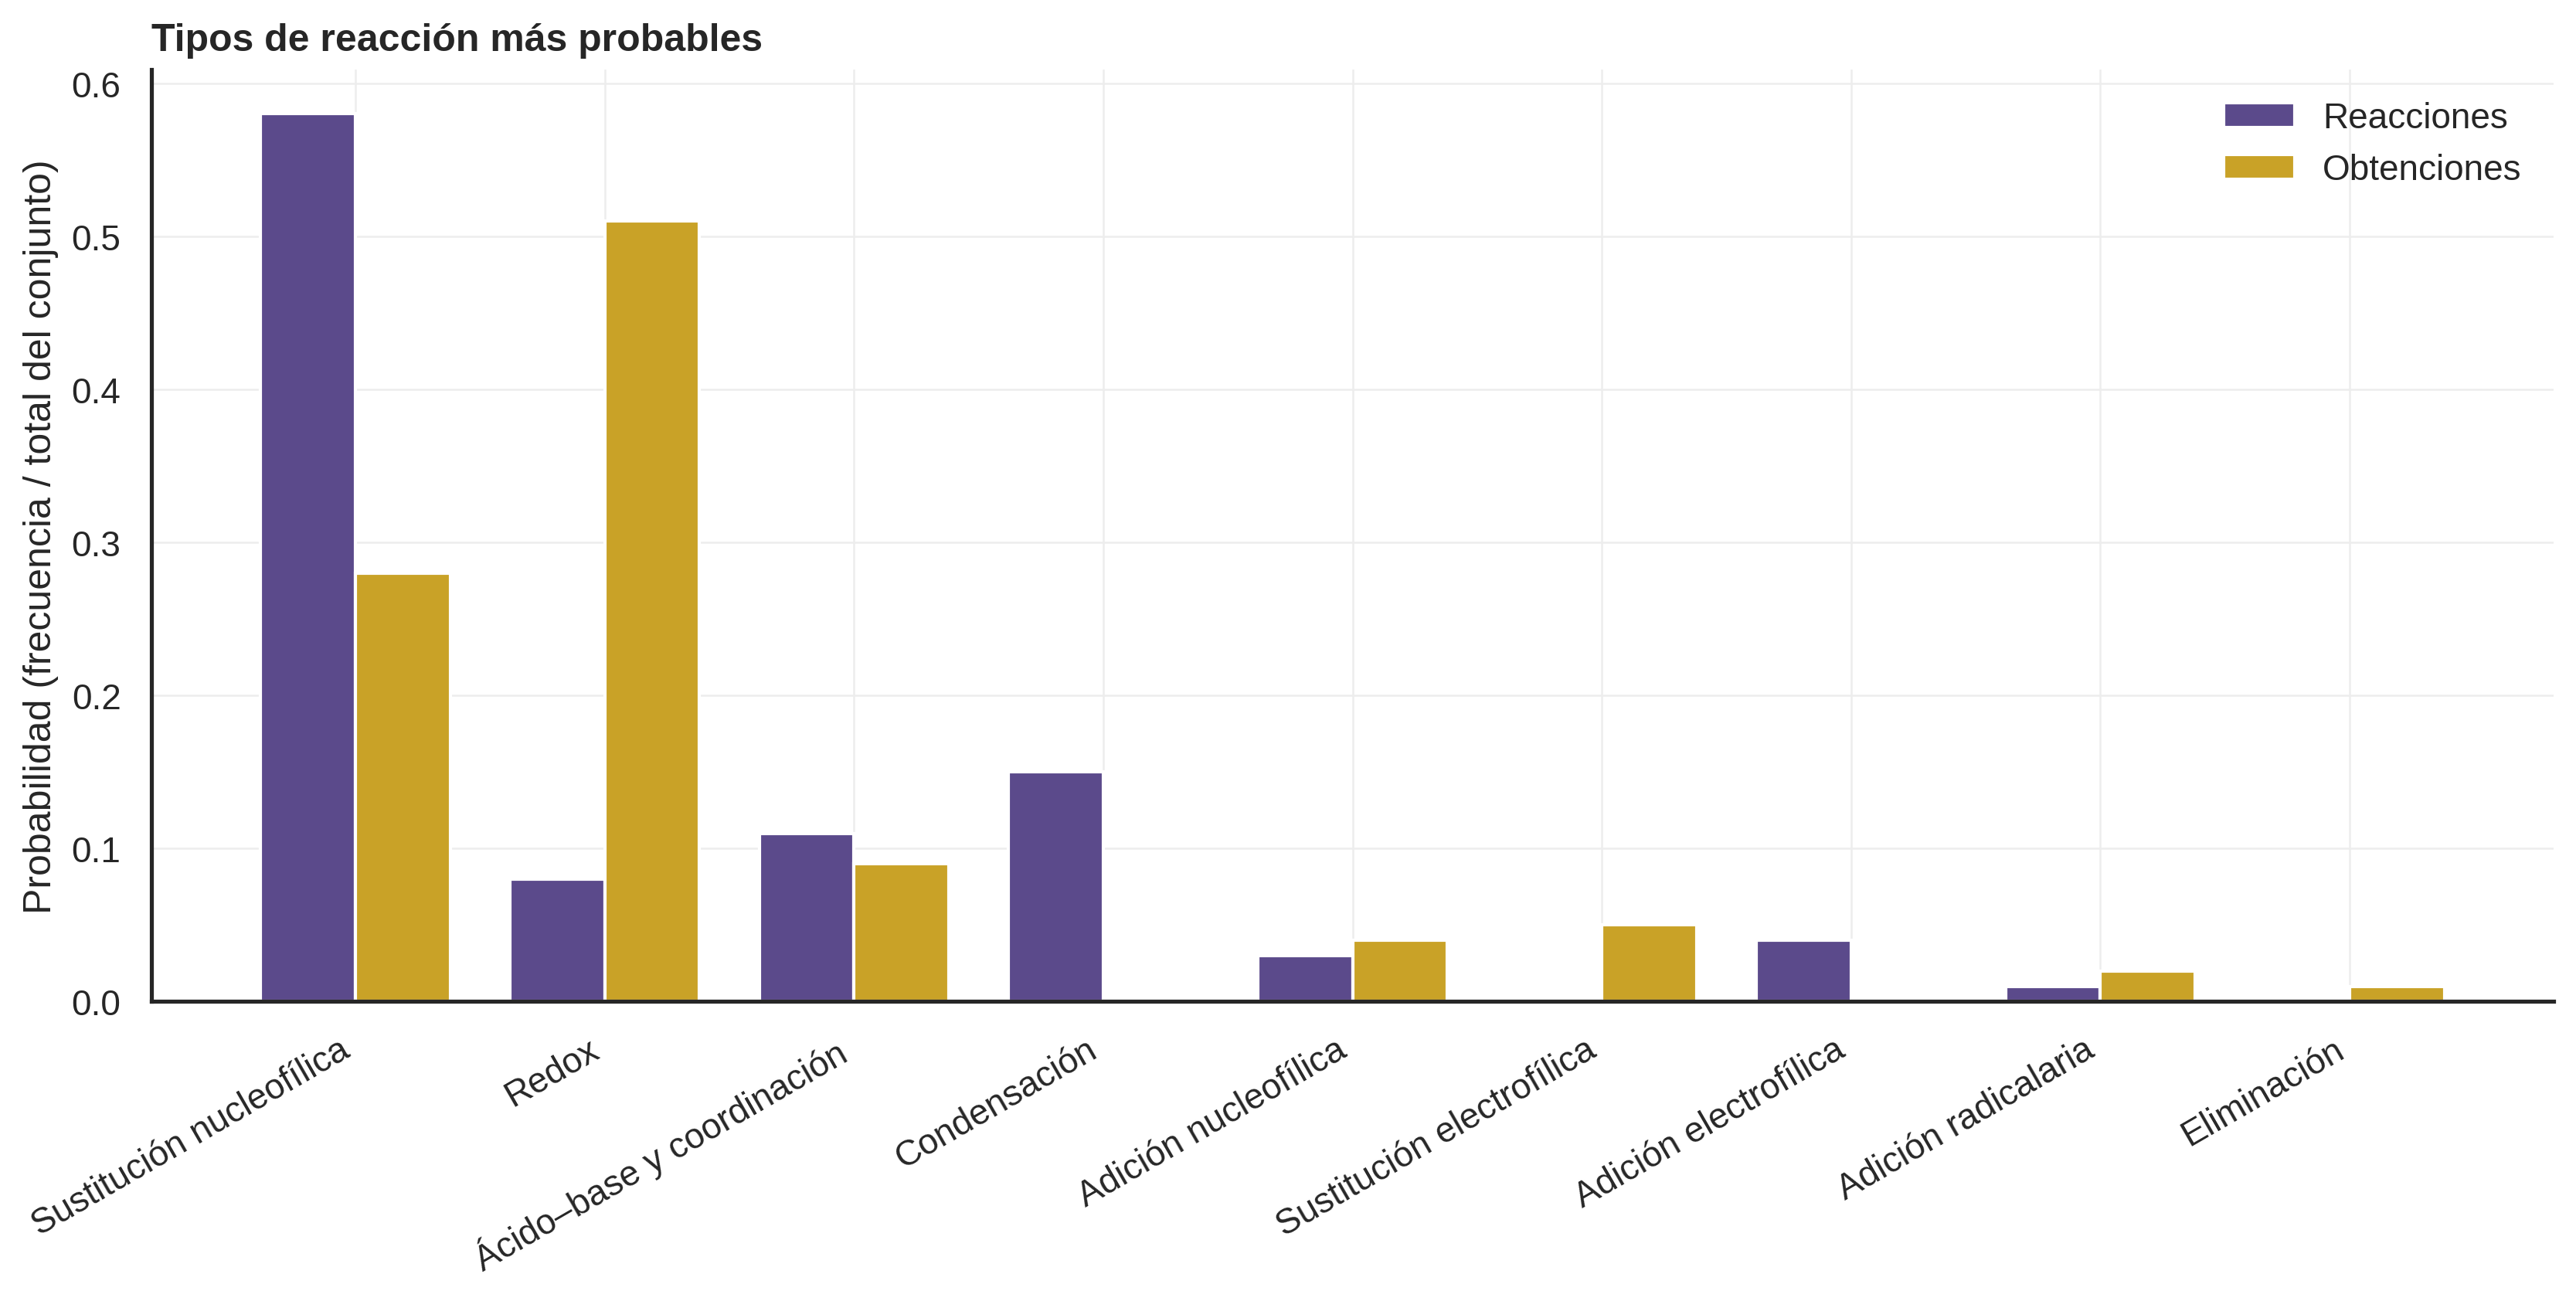
\includegraphics[width=\linewidth]{12_tipos_reaccion.png}
\caption{Tipo de reacción (por mecanismo).}
\label{fig:tipos}
\end{subfigure}\hfill
\begin{subfigure}[t]{0.42\textwidth}\centering
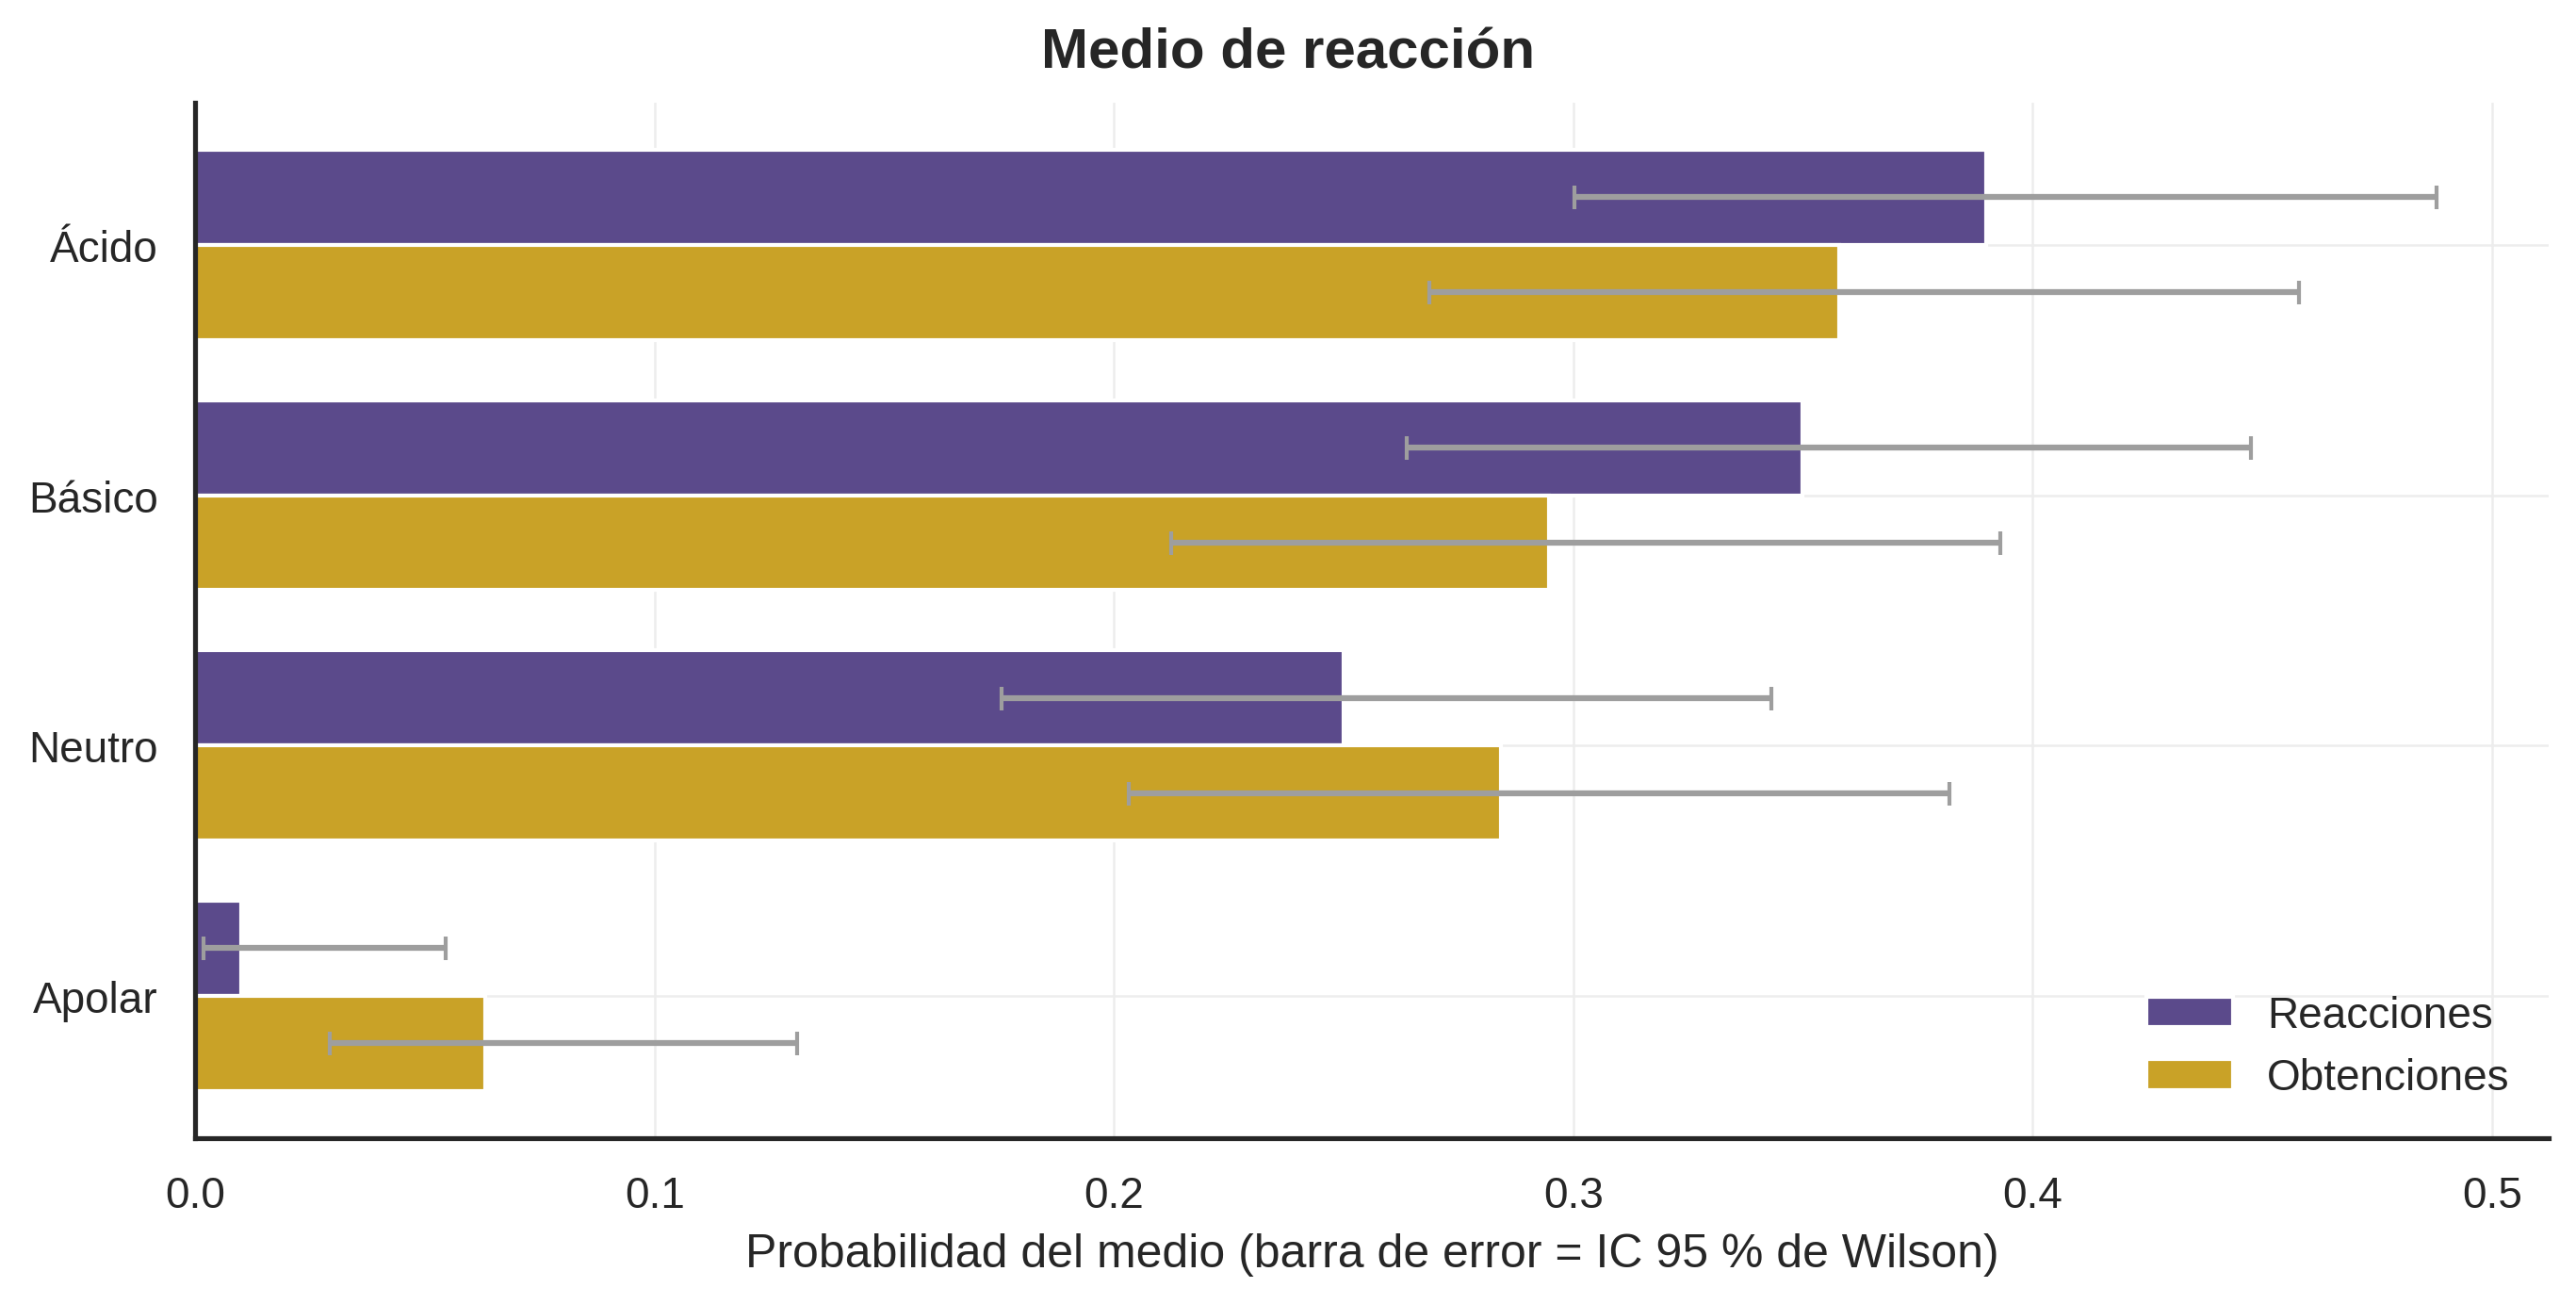
\includegraphics[width=\linewidth]{13_medio_reaccion.png}
\caption{Medio de reacción, con IC 95\,\% de Wilson.}
\label{fig:medio}
\end{subfigure}
\caption{Probabilidad de cada tipo de reacción y de cada medio en las reacciones (el ácido como reactivo) y en las obtenciones (el ácido como producto).}
\label{fig:tiposmedio}
\end{figure*}

Cuando los ácidos reaccionan, domina la sustitución nucleofílica (58\,\%; Figura~\ref{fig:tipos}): el grupo carboxilo, o su derivado activado, forma ésteres y amidas. Le sigue la condensación (15\,\%). En las obtenciones domina el redox (51\,\%), que incluye la oxidación de alcoholes y aldehídos, la hidrogenación de dobles enlaces y las fermentaciones, seguido de la sustitución nucleofílica (28\,\%), que corresponde a la hidrólisis de ésteres, amidas y haluros de acilo.

Los medios ácido (0.39 en reacciones y 0.36 en obtenciones) y básico (0.35 y 0.29) son los más probables (Figura~\ref{fig:medio}) y el medio apolar es poco frecuente (0.01 y 0.06).

\begin{figure*}[!t]
\centering
\begin{subfigure}[t]{0.47\textwidth}\centering
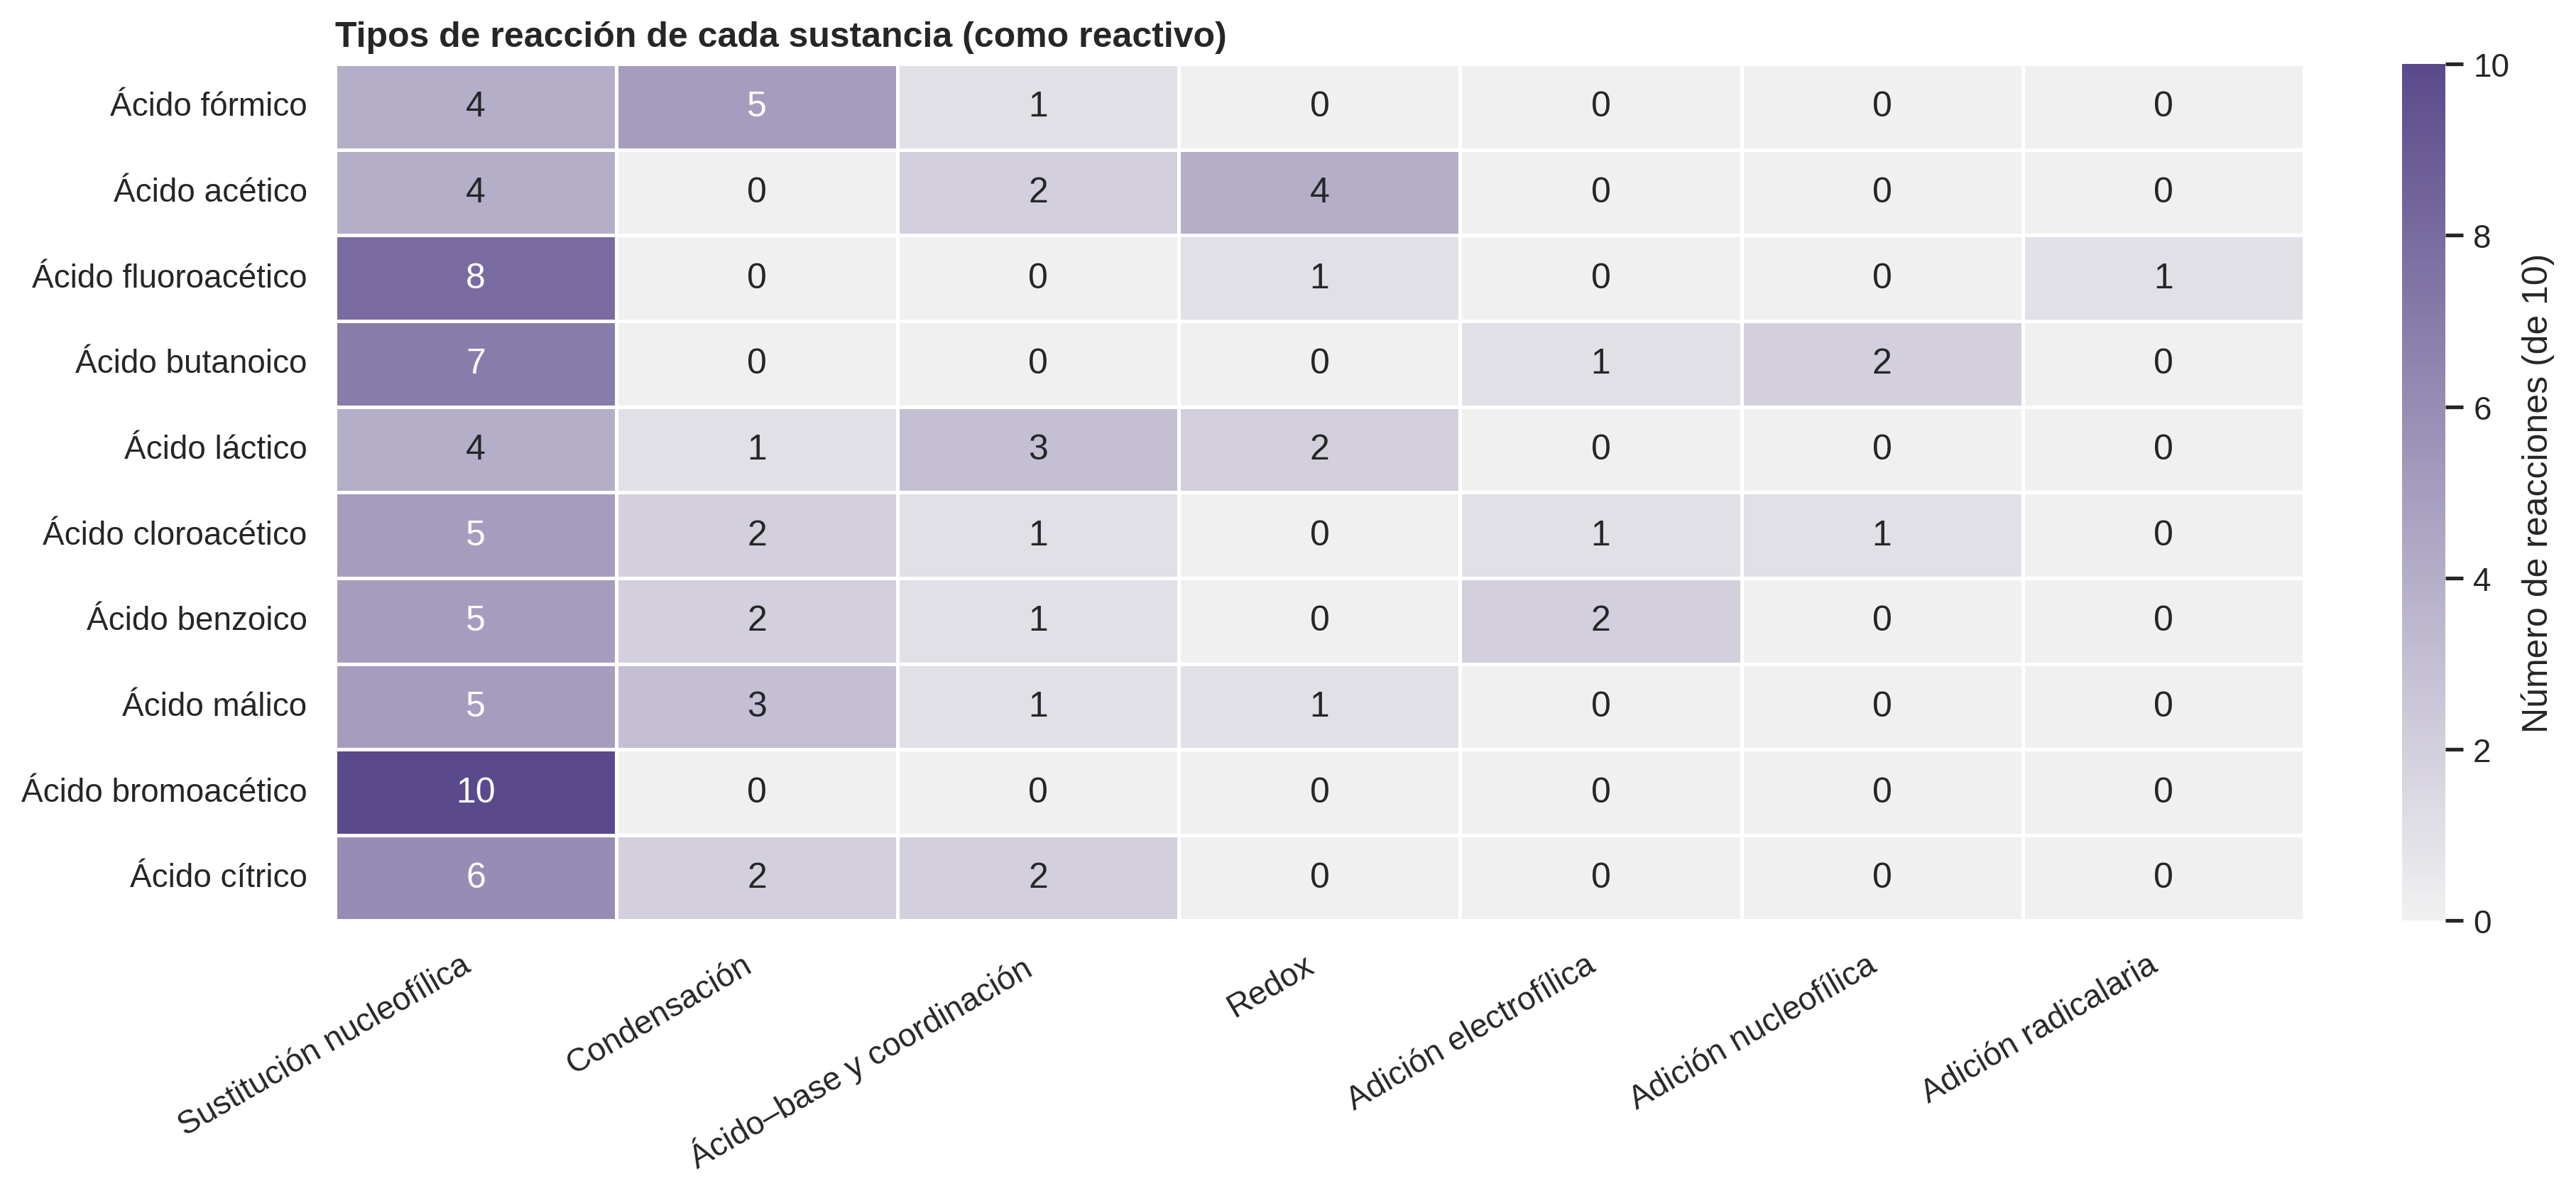
\includegraphics[width=\linewidth]{15_sustancia_tipo.png}
\caption{Tipo de reacción de cada ácido (como reactivo).}
\label{fig:sustipo}
\end{subfigure}\hfill
\begin{subfigure}[t]{0.51\textwidth}\centering
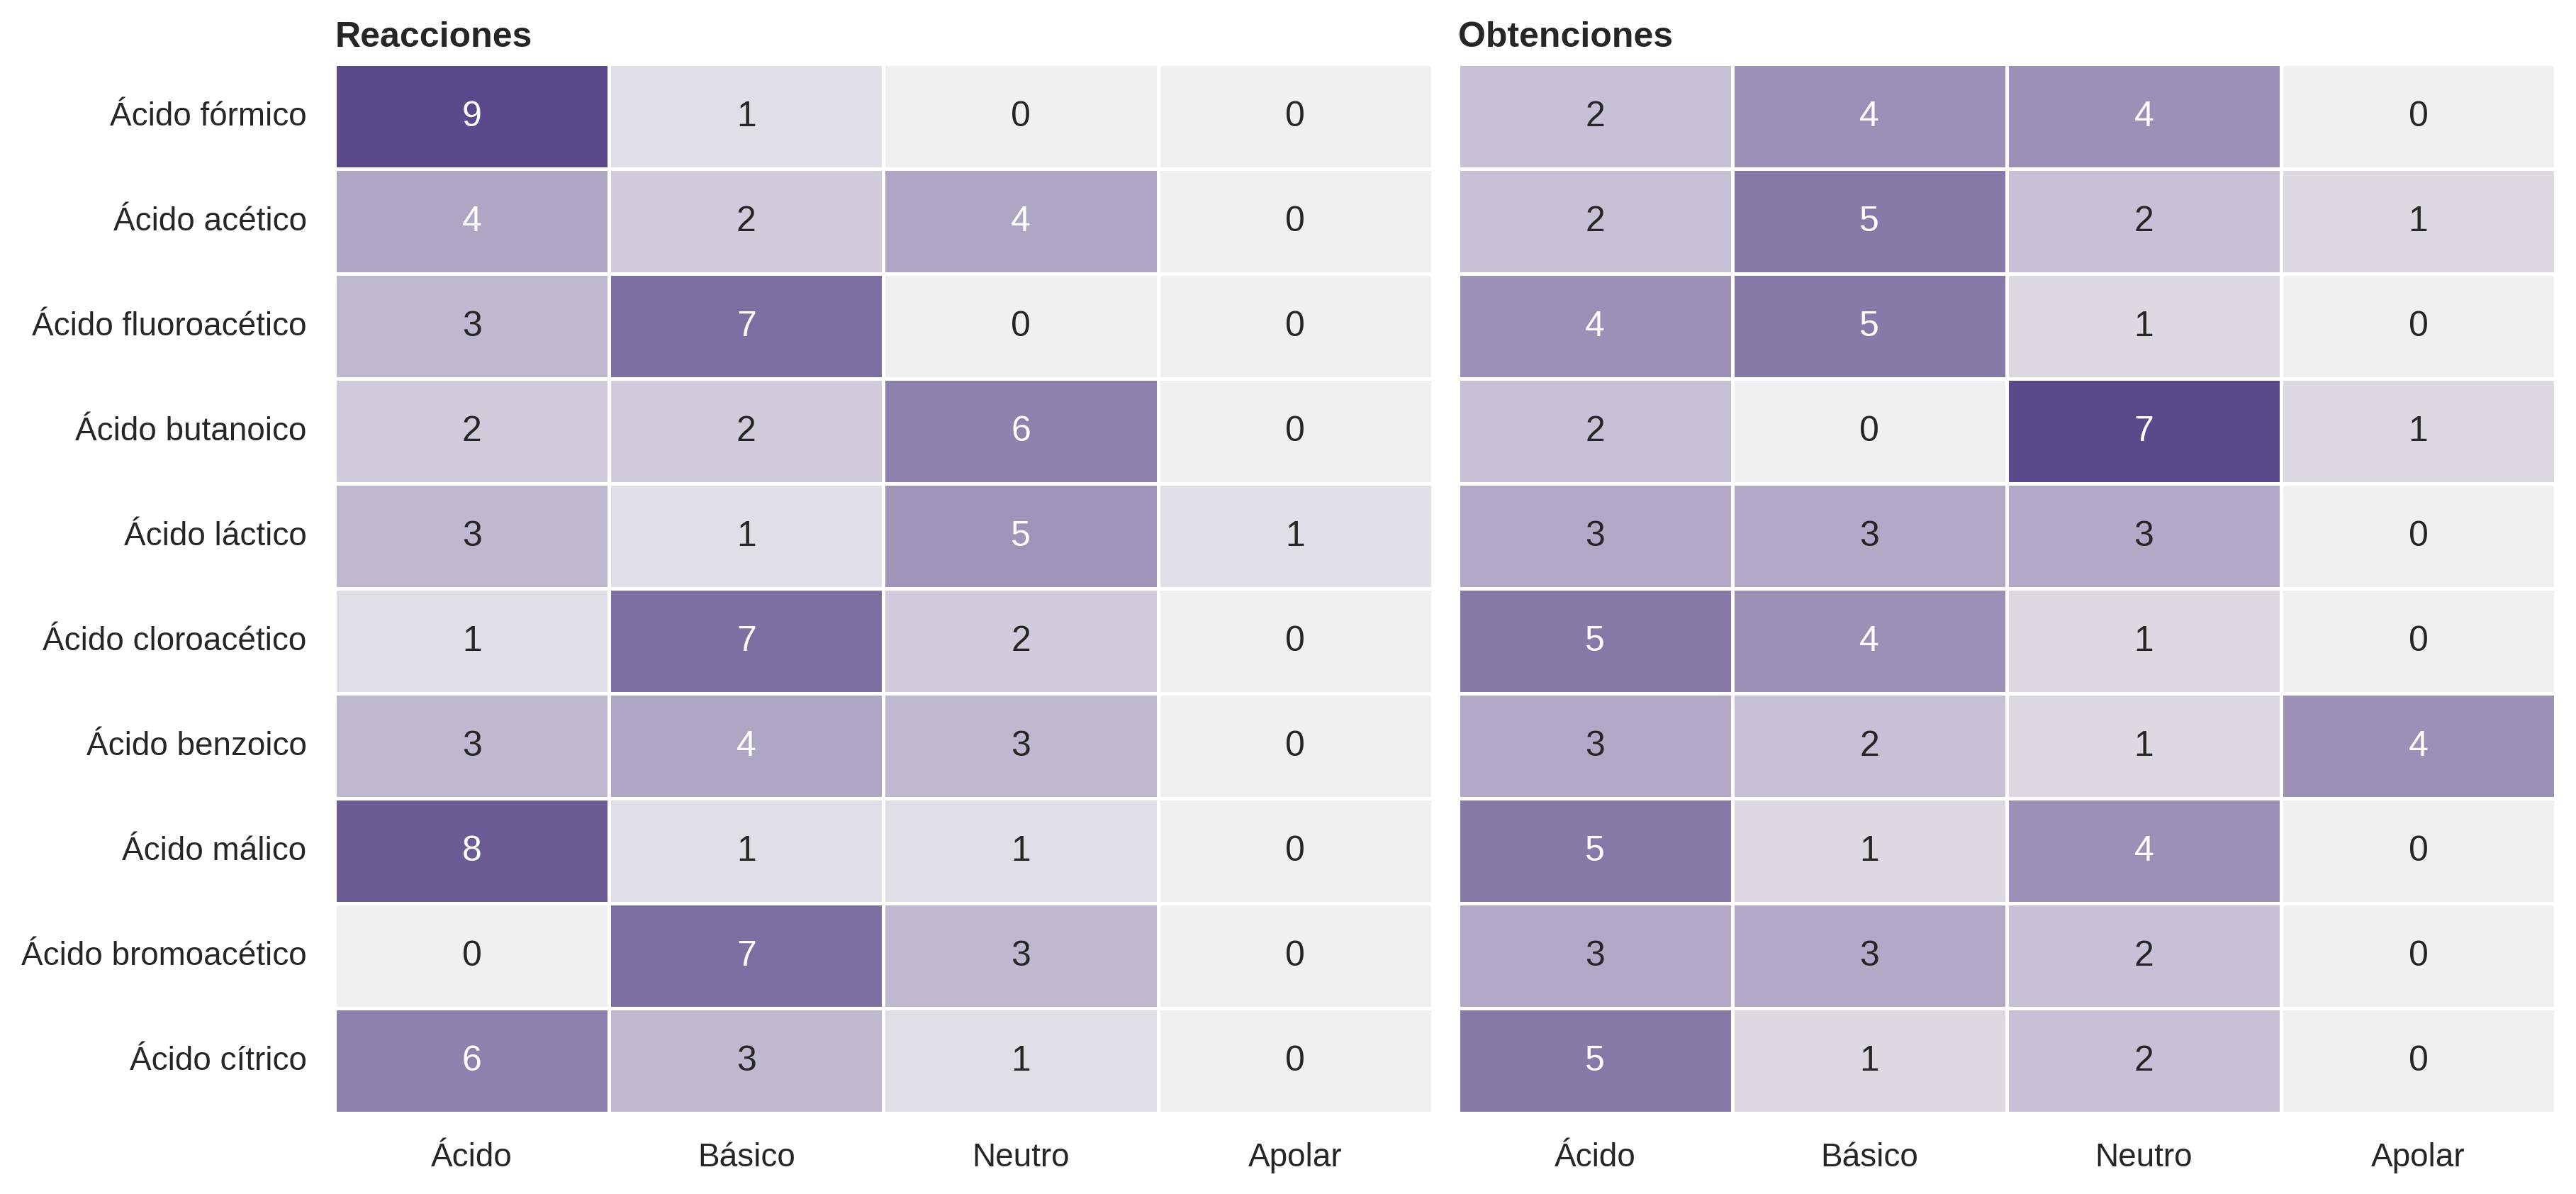
\includegraphics[width=\linewidth]{14_sustancia_medio.png}
\caption{Medio de reacción de cada ácido.}
\label{fig:susmedio}
\end{subfigure}
\caption{Número de reacciones de cada ácido por tipo de reacción (a) y por medio (b). En (b), el panel izquierdo corresponde a reacciones y el derecho a obtenciones.}
\label{fig:sustancias}
\end{figure*}

La Figura~\ref{fig:sustipo} muestra que el ácido bromoacético reacciona por sustitución nucleofílica en sus diez reacciones, porque el bromo en el carbono $\alpha$ es un buen grupo saliente; el fluoroacético (8) y el butanoico (7) reaccionan sobre todo por sustitución nucleofílica en el acilo, y el fórmico es el que más reacciones de condensación presenta (5). Por medio (Figura~\ref{fig:susmedio}), el fórmico reacciona en medio ácido en 9 de 10 casos, mientras que los tres haloácidos lo hacen en medio básico en 7 de 10, porque la base activa al nucleófilo que desplaza al halógeno.

\subsection{Condiciones de reacción}

\begin{figure*}[!t]
\centering
\begin{subfigure}[t]{0.47\textwidth}\centering
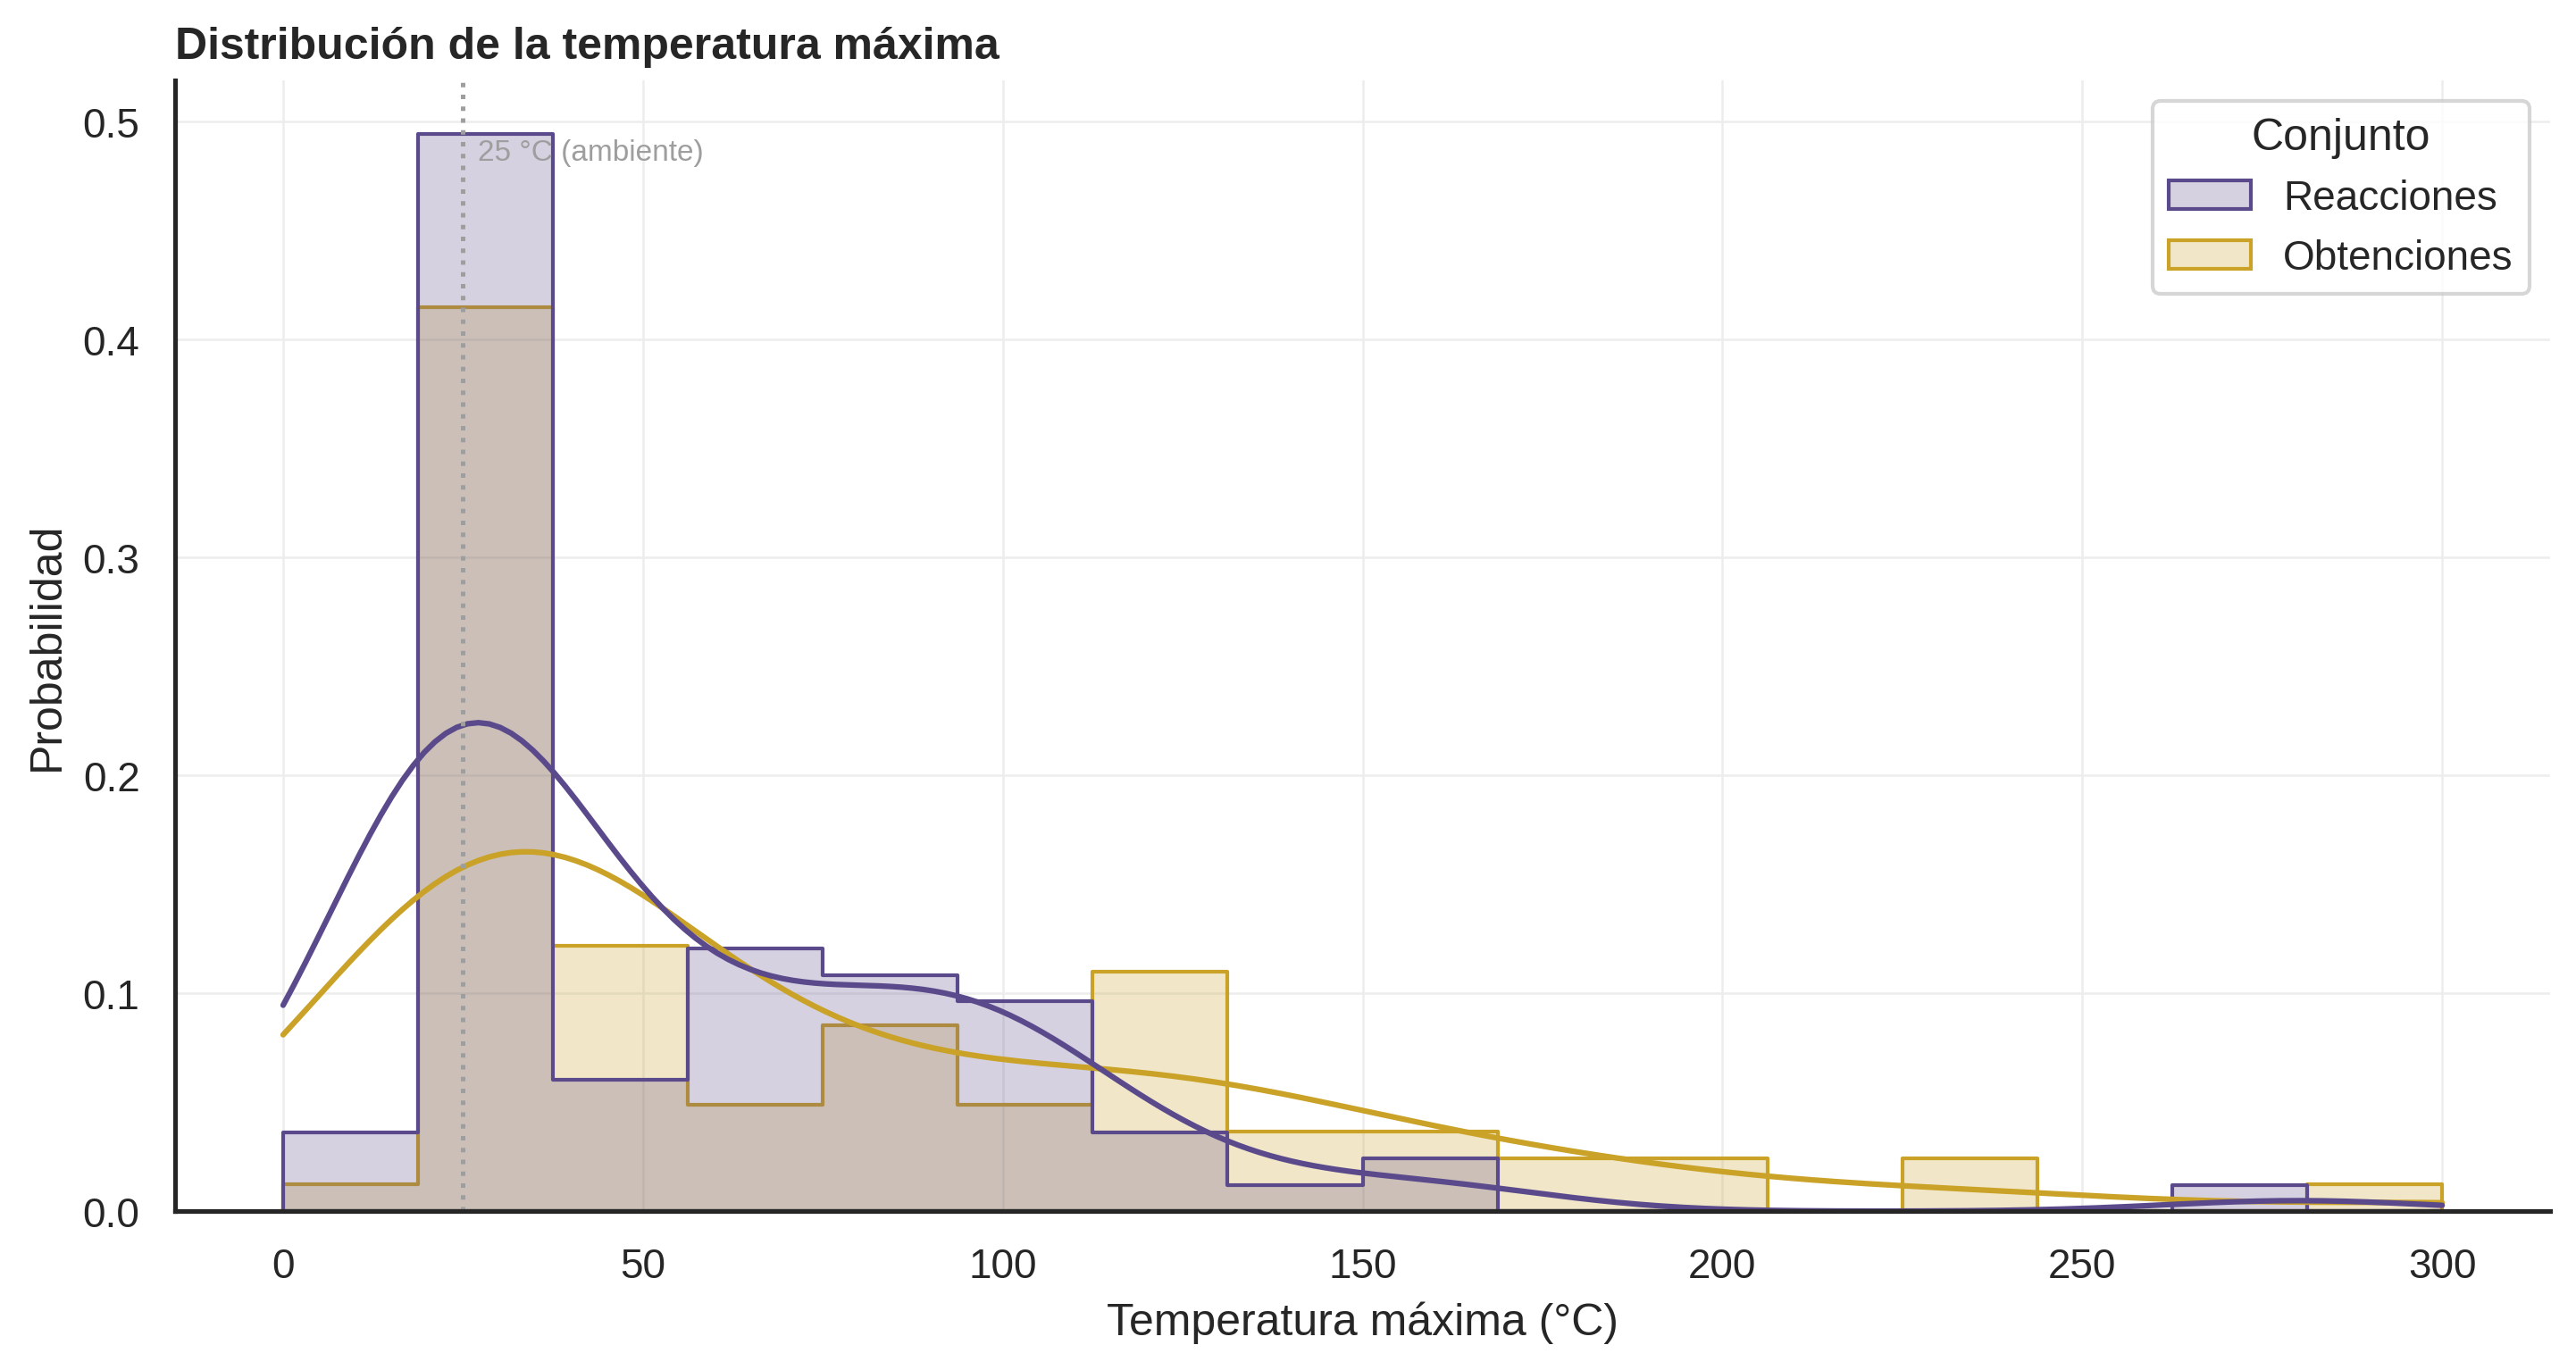
\includegraphics[width=\linewidth]{02_distribucion_temperatura.png}
\caption{Distribución de la temperatura máxima.}
\label{fig:temp}
\end{subfigure}\hfill
\begin{subfigure}[t]{0.51\textwidth}\centering
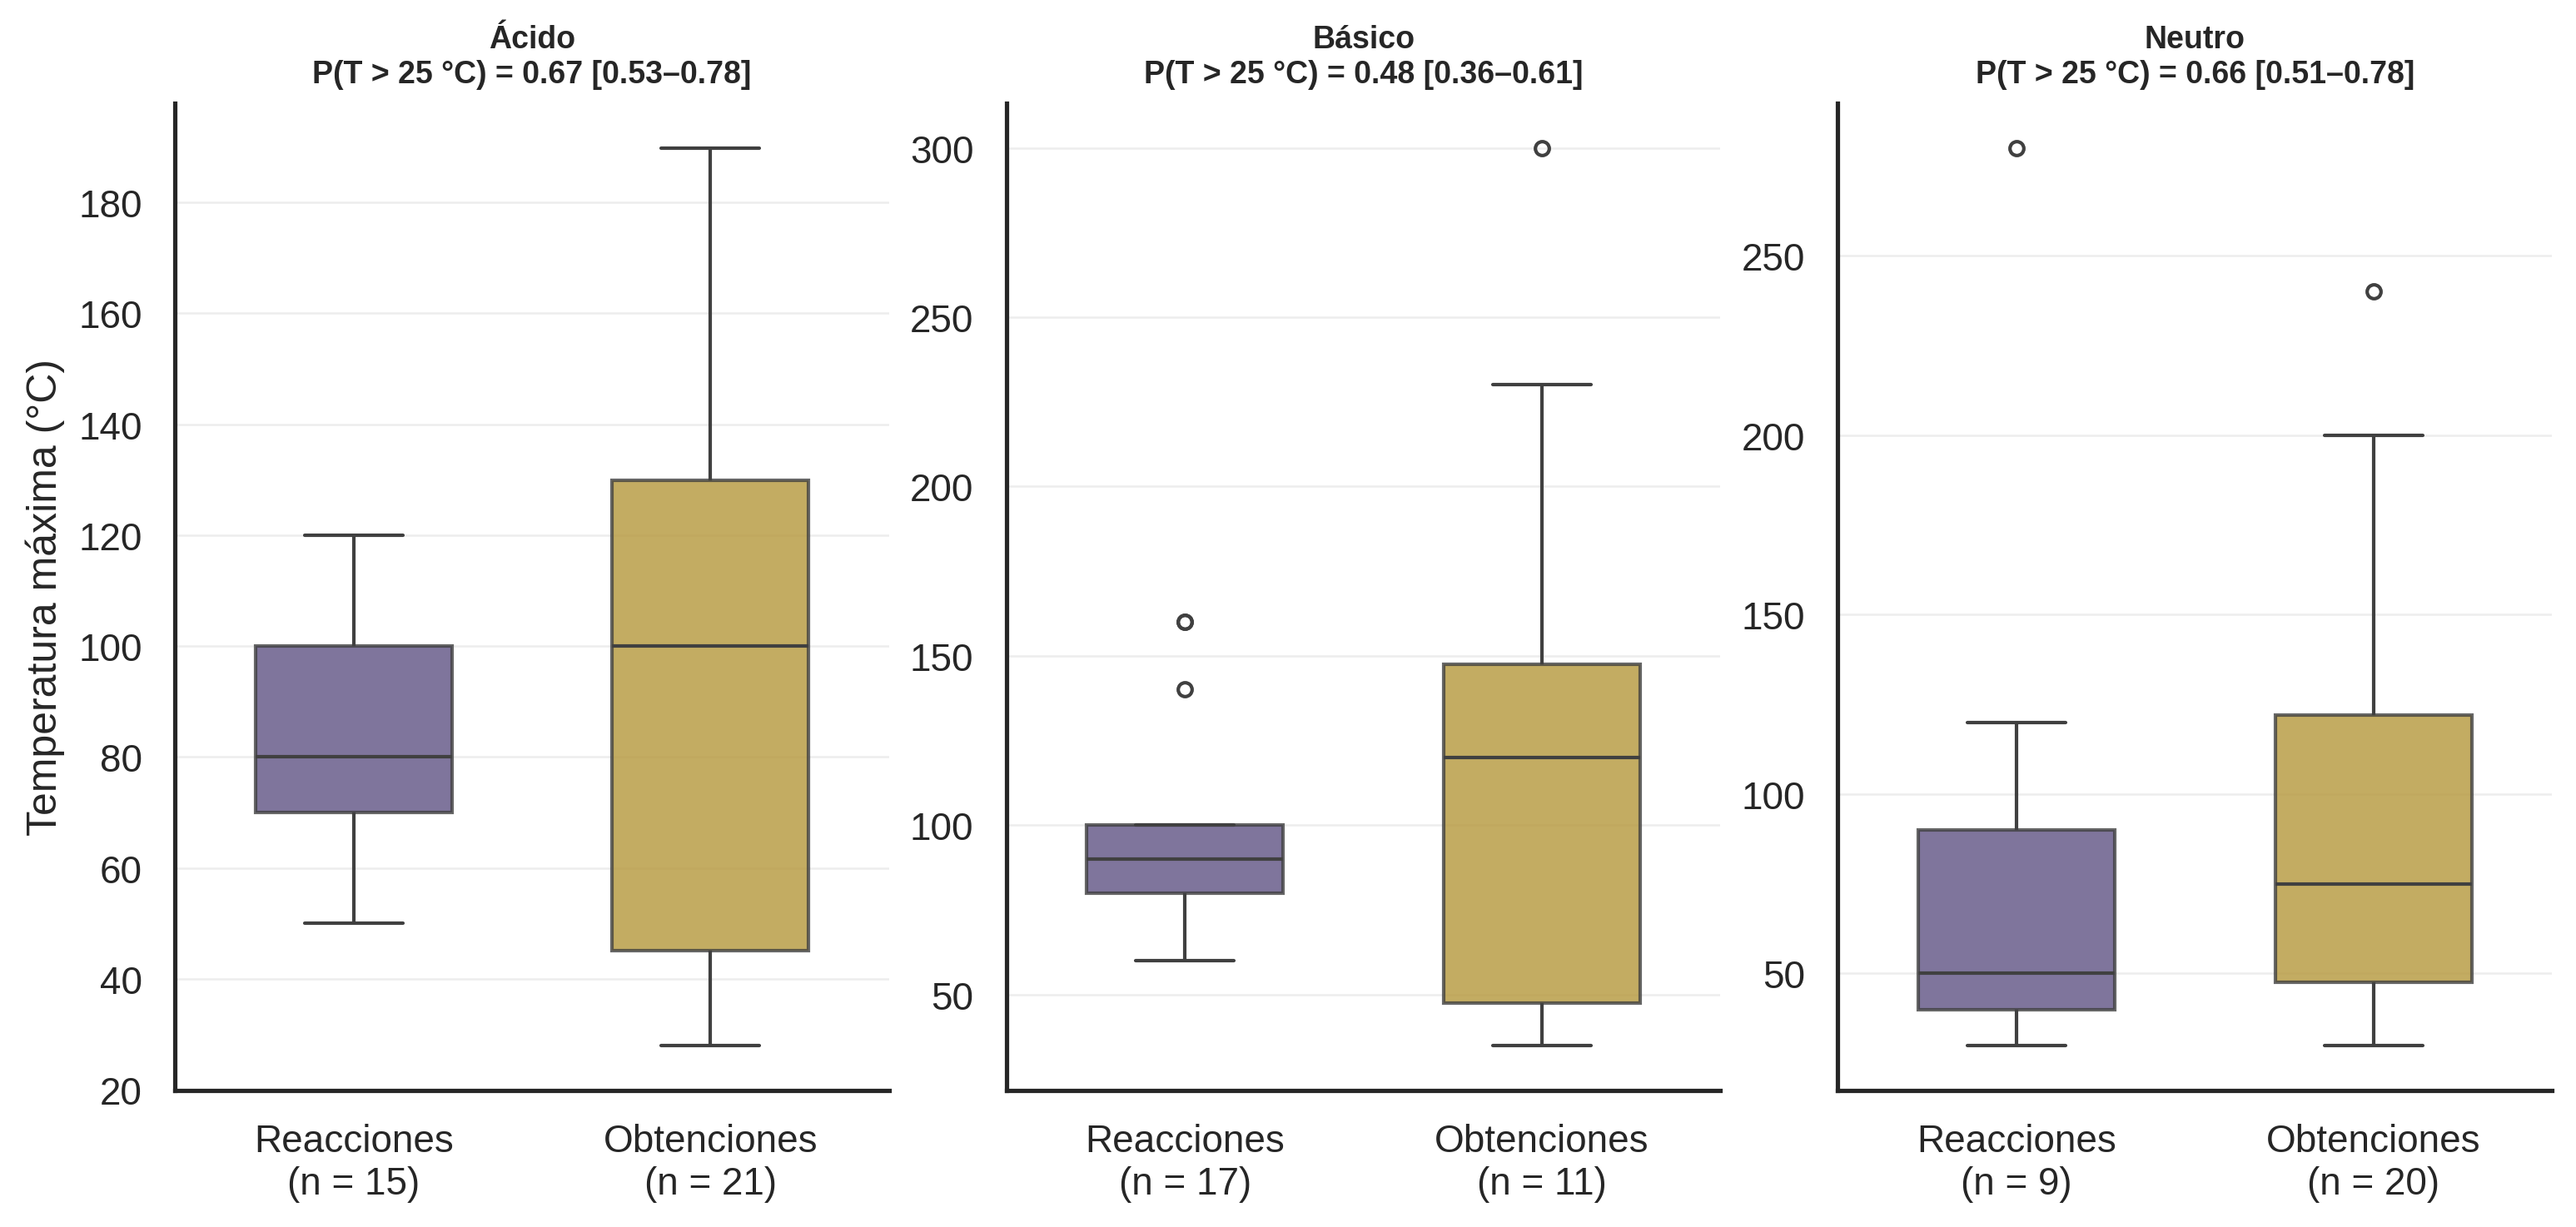
\includegraphics[width=\linewidth]{03_temperatura_por_medio.png}
\caption{Temperatura de las reacciones con calentamiento, por medio.}
\label{fig:tempmedio}
\end{subfigure}
\caption{Temperatura de reacción. En (a) la línea punteada marca 25~\textdegree C; en (b) solo se incluyen reacciones con T $>$ 25~\textdegree C y cajas con al menos cinco datos.}
\label{fig:temperatura}
\end{figure*}

Las obtenciones requieren calentamiento con mayor probabilidad que las reacciones: P(T~$>$~25~\textdegree C) = 0.68 [0.58–0.77] frente a 0.49 [0.39–0.60], con medianas de 45 y 25~\textdegree C (Figura~\ref{fig:temp}), ya que oxidar o hidrolizar para formar el grupo –COOH suele requerir más energía que transformarlo. En medio ácido se calienta con frecuencia (P = 0.67), con medianas de 80~\textdegree C en reacciones y 100~\textdegree C en obtenciones (Figura~\ref{fig:tempmedio}), lo que es coherente con la esterificación de Fischer, un equilibrio que se favorece con calor y eliminación de agua \cite{Mannu2024}. En medio básico la probabilidad de calentamiento es menor (0.48) y, cuando se calienta, se alcanzan medianas de 90 y 120~\textdegree C.

\begin{figure*}[!t]
\centering
\begin{subfigure}[t]{0.49\textwidth}\centering
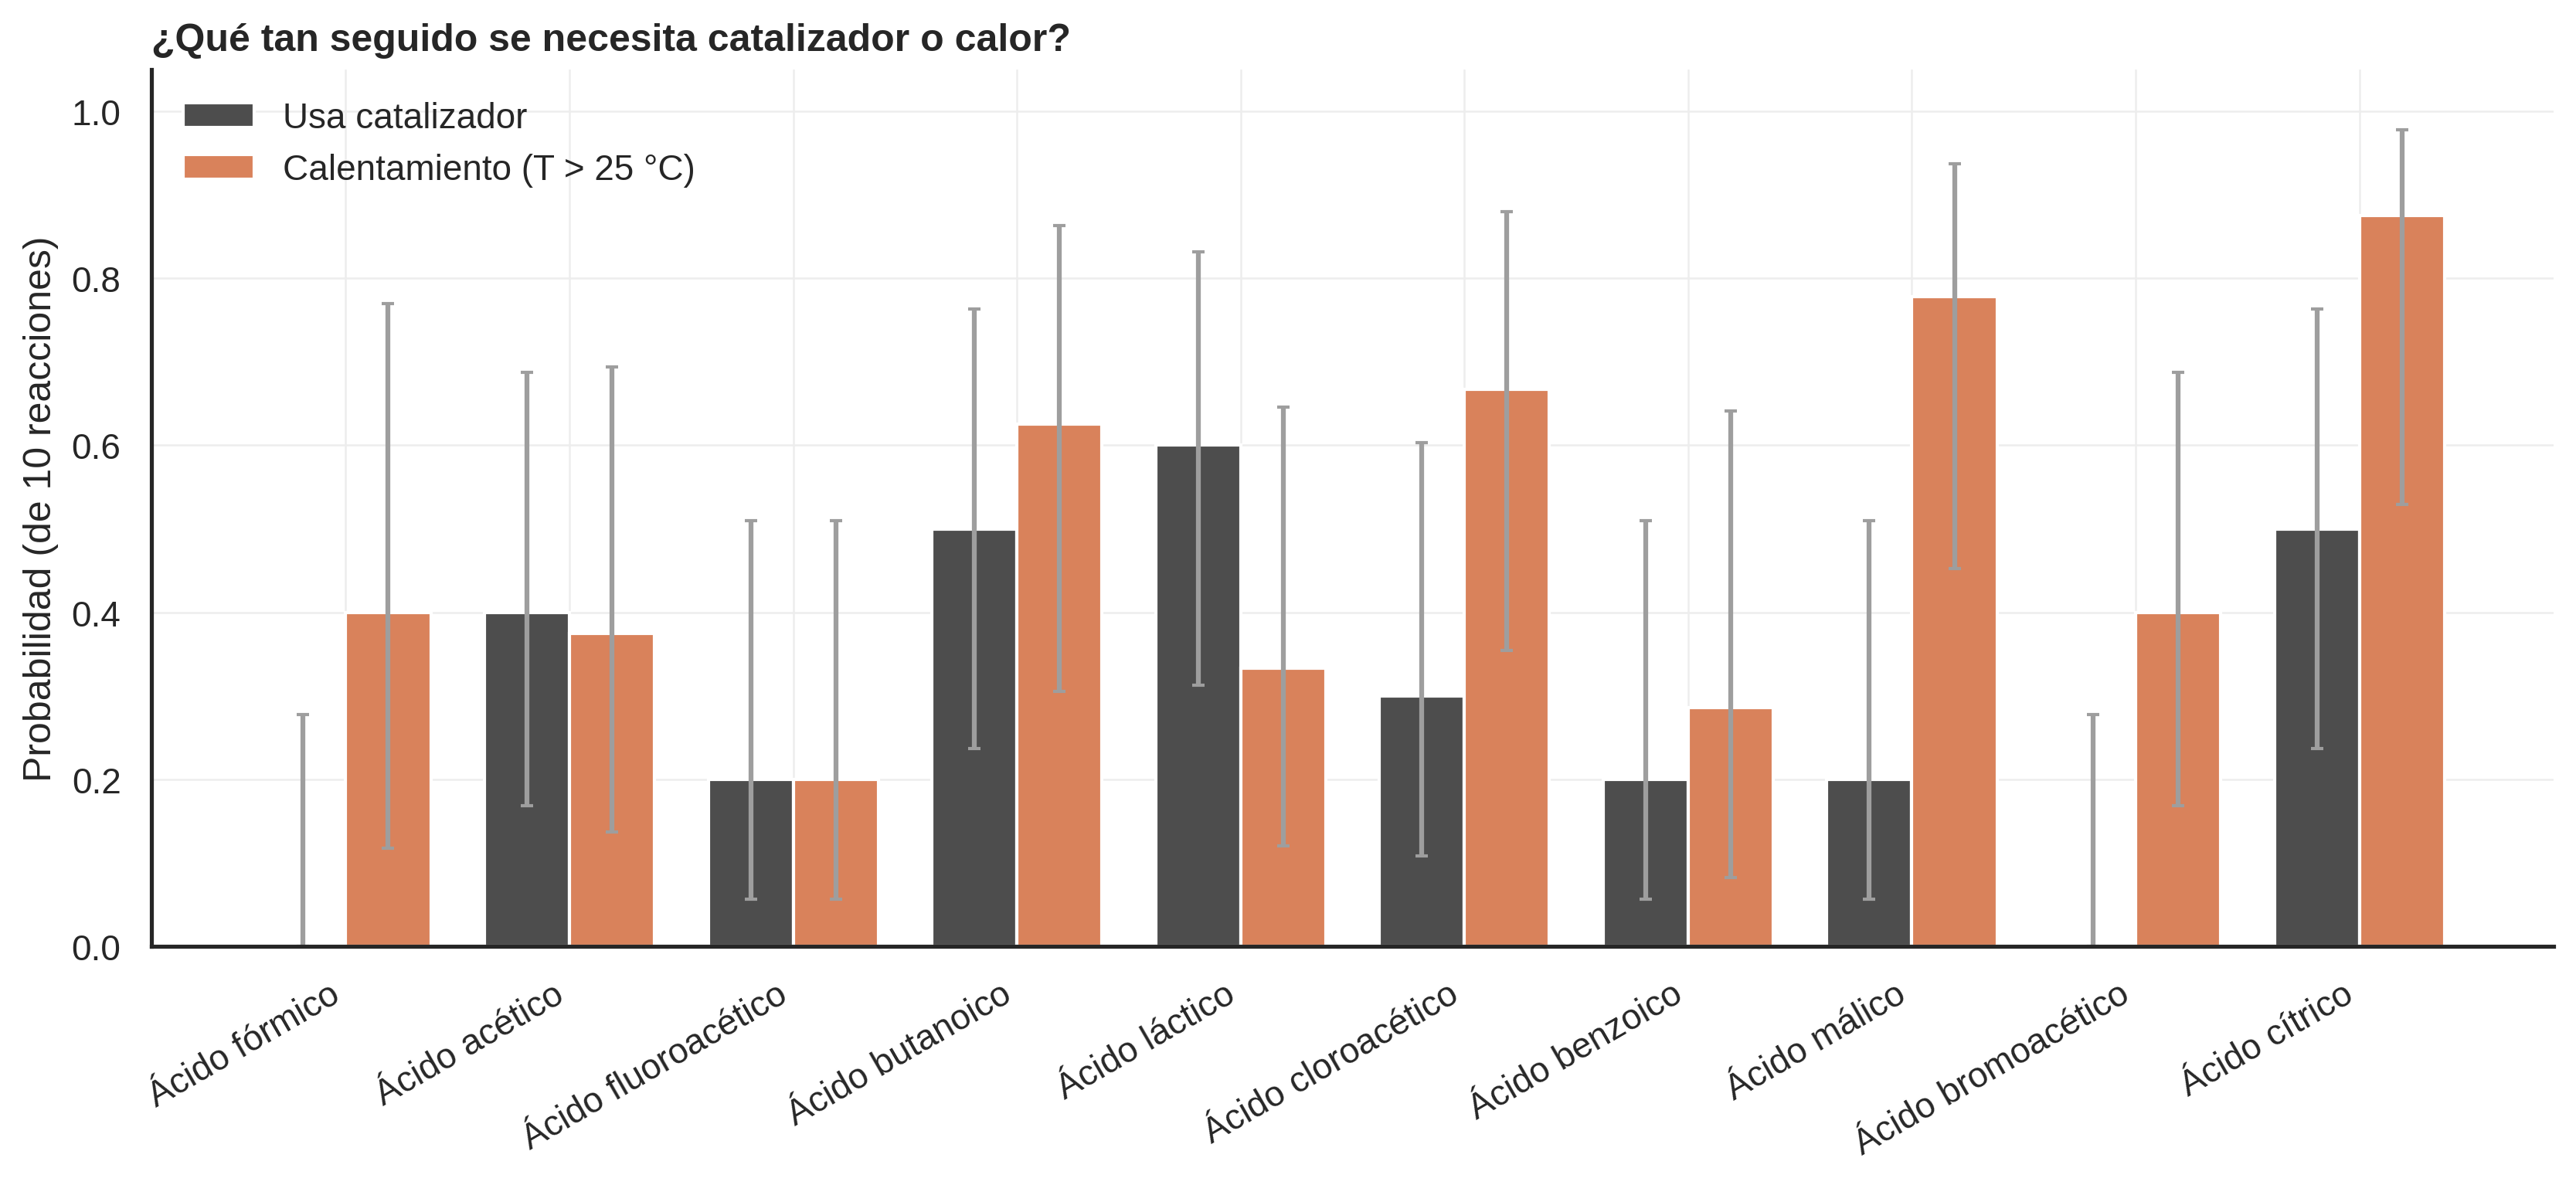
\includegraphics[width=\linewidth]{17_prob_catalizador_calor.png}
\caption{Probabilidad de usar catalizador y de calentar, con IC 95\,\% de Wilson.}
\label{fig:catcalor}
\end{subfigure}\hfill
\begin{subfigure}[t]{0.49\textwidth}\centering
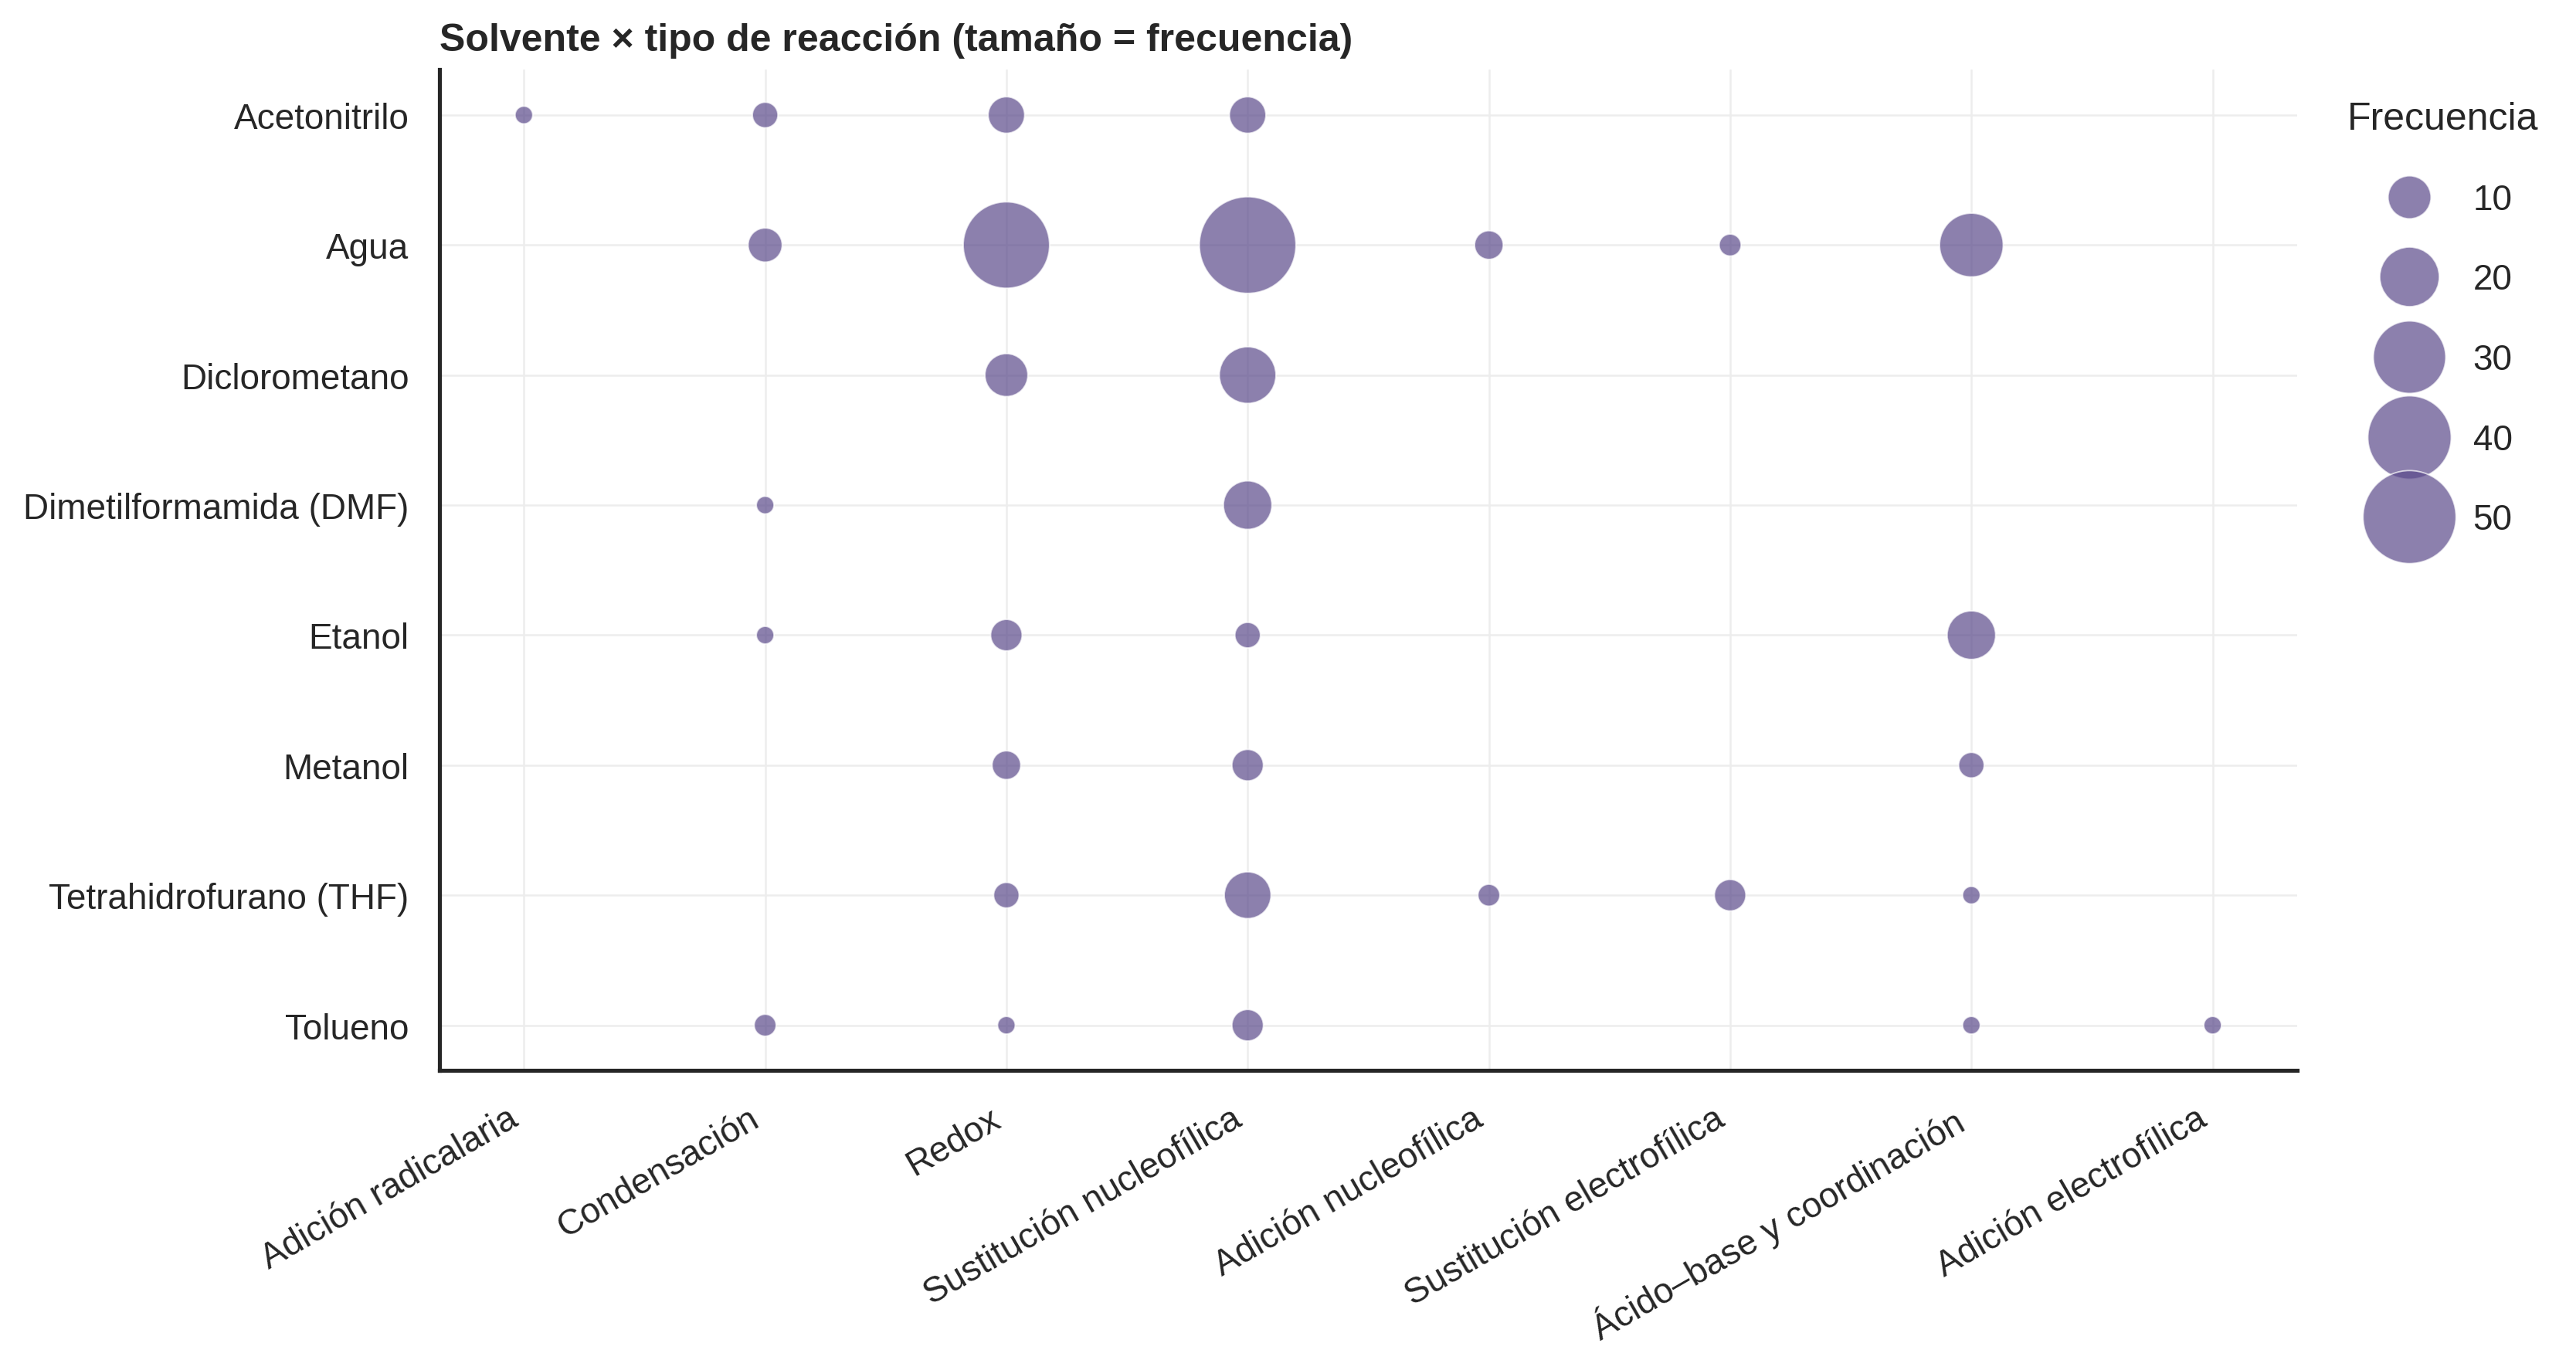
\includegraphics[width=\linewidth]{16_burbujas_solvente_tipo.png}
\caption{Solvente frente a tipo de reacción (8 solventes más usados).}
\label{fig:burbujas}
\end{subfigure}
\caption{Condiciones de las reacciones de cada ácido: catalizador y calentamiento (a) y solventes (b).}
\label{fig:condiciones}
\end{figure*}

El catalizador se usa en el 29\,\% de las reacciones y es más probable cuando hay calentamiento (0.41, $n$ = 41) que cuando no lo hay (0.24, $n$ = 42; Figura~\ref{fig:catcalor}). Se observa que el ácido cítrico es el que más se calienta (7 de 8 reacciones con temperatura conocida), mientras que el fórmico y el bromoacético no usan catalizador en ninguna de sus reacciones registradas en este ejercicio.

El agua es el solvente más usado, sobre todo en sustitución nucleofílica (54 casos), redox (43) y reacciones ácido--base (23), lo que refleja la solubilidad de los ácidos de cadena corta y el papel del agua como reactivo en las hidrólisis (Figura~\ref{fig:burbujas}). El diclorometano, en cambio, aparece principalmente en la formación de amidas, que se realiza en solventes orgánicos sin agua. Estas relaciones se observan mejor en el cuaderno de Colab, cuyas gráficas interactivas (Figura~\ref{fig:interactivas}) permiten explorar cada producto y la jerarquía sustancia–medio–tipo de reacción.

\begin{figure*}[!t]
\centering
\begin{subfigure}[t]{0.49\textwidth}\centering
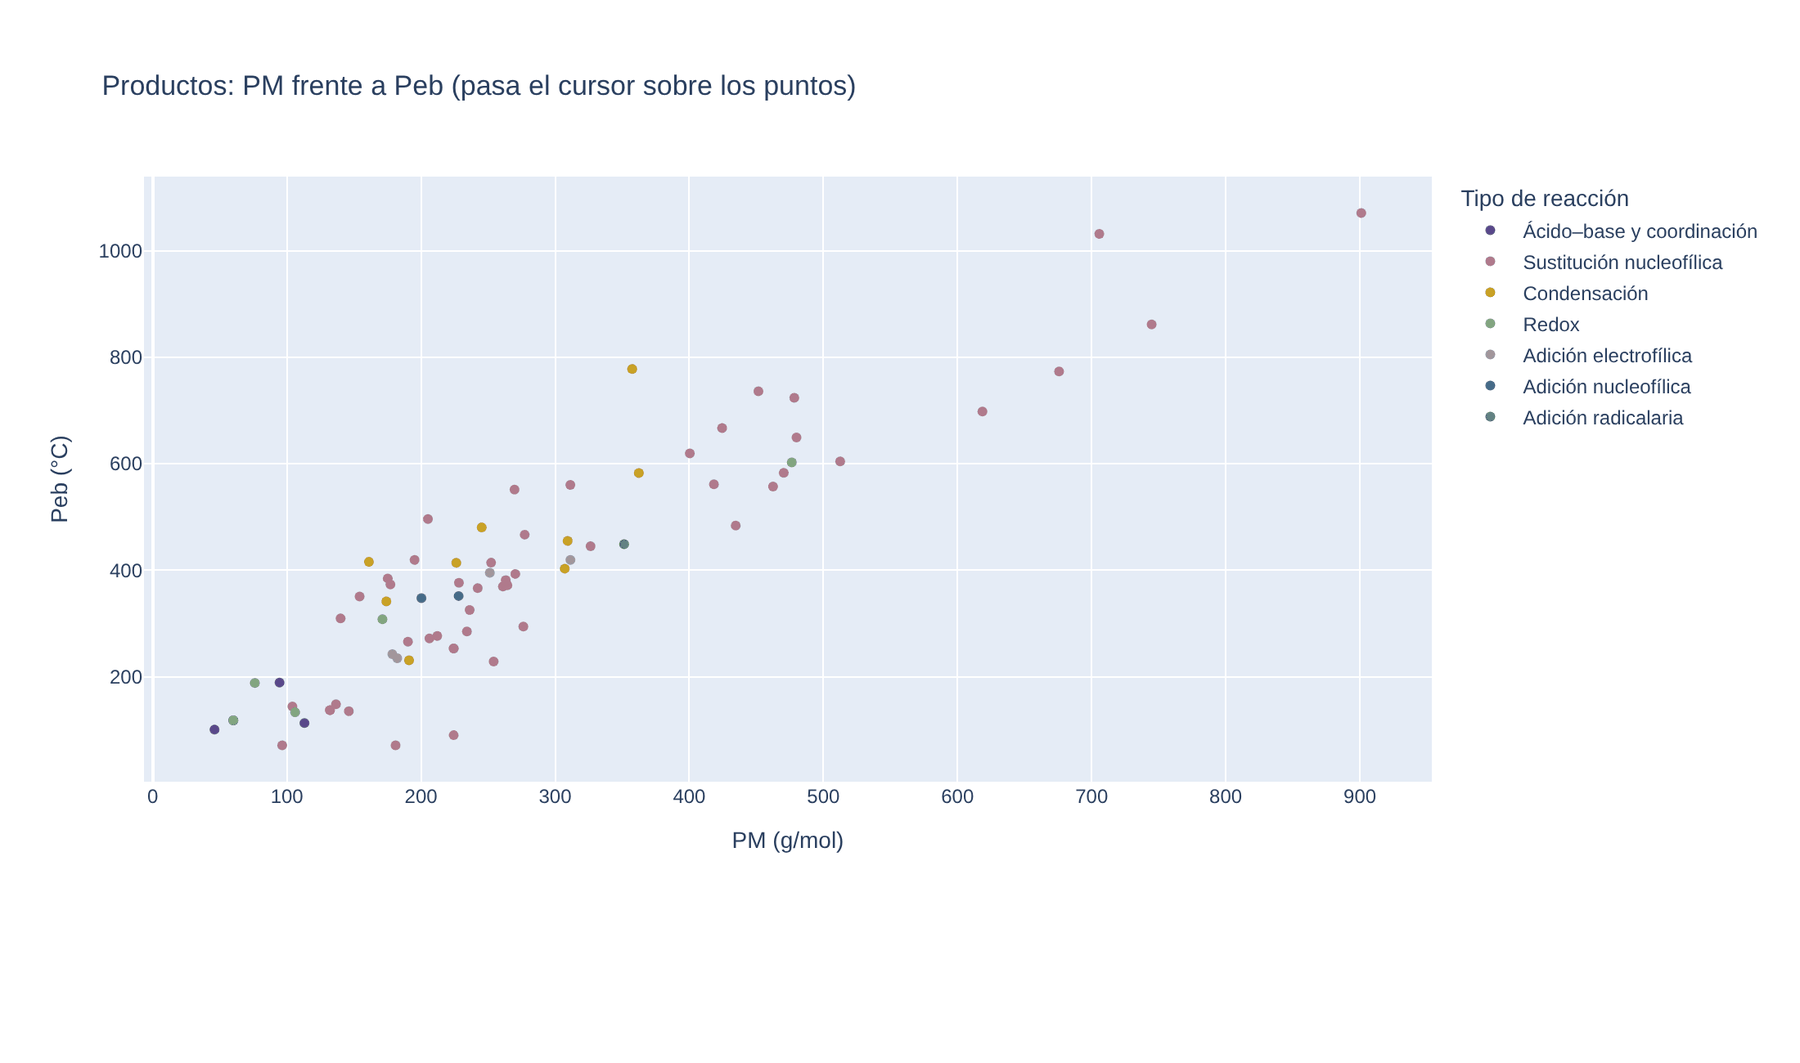
\includegraphics[width=\linewidth]{18_interactivo_PM_Peb.png}
\caption{Dispersión PM–Peb por tipo de reacción.}
\end{subfigure}\hfill
\begin{subfigure}[t]{0.49\textwidth}\centering
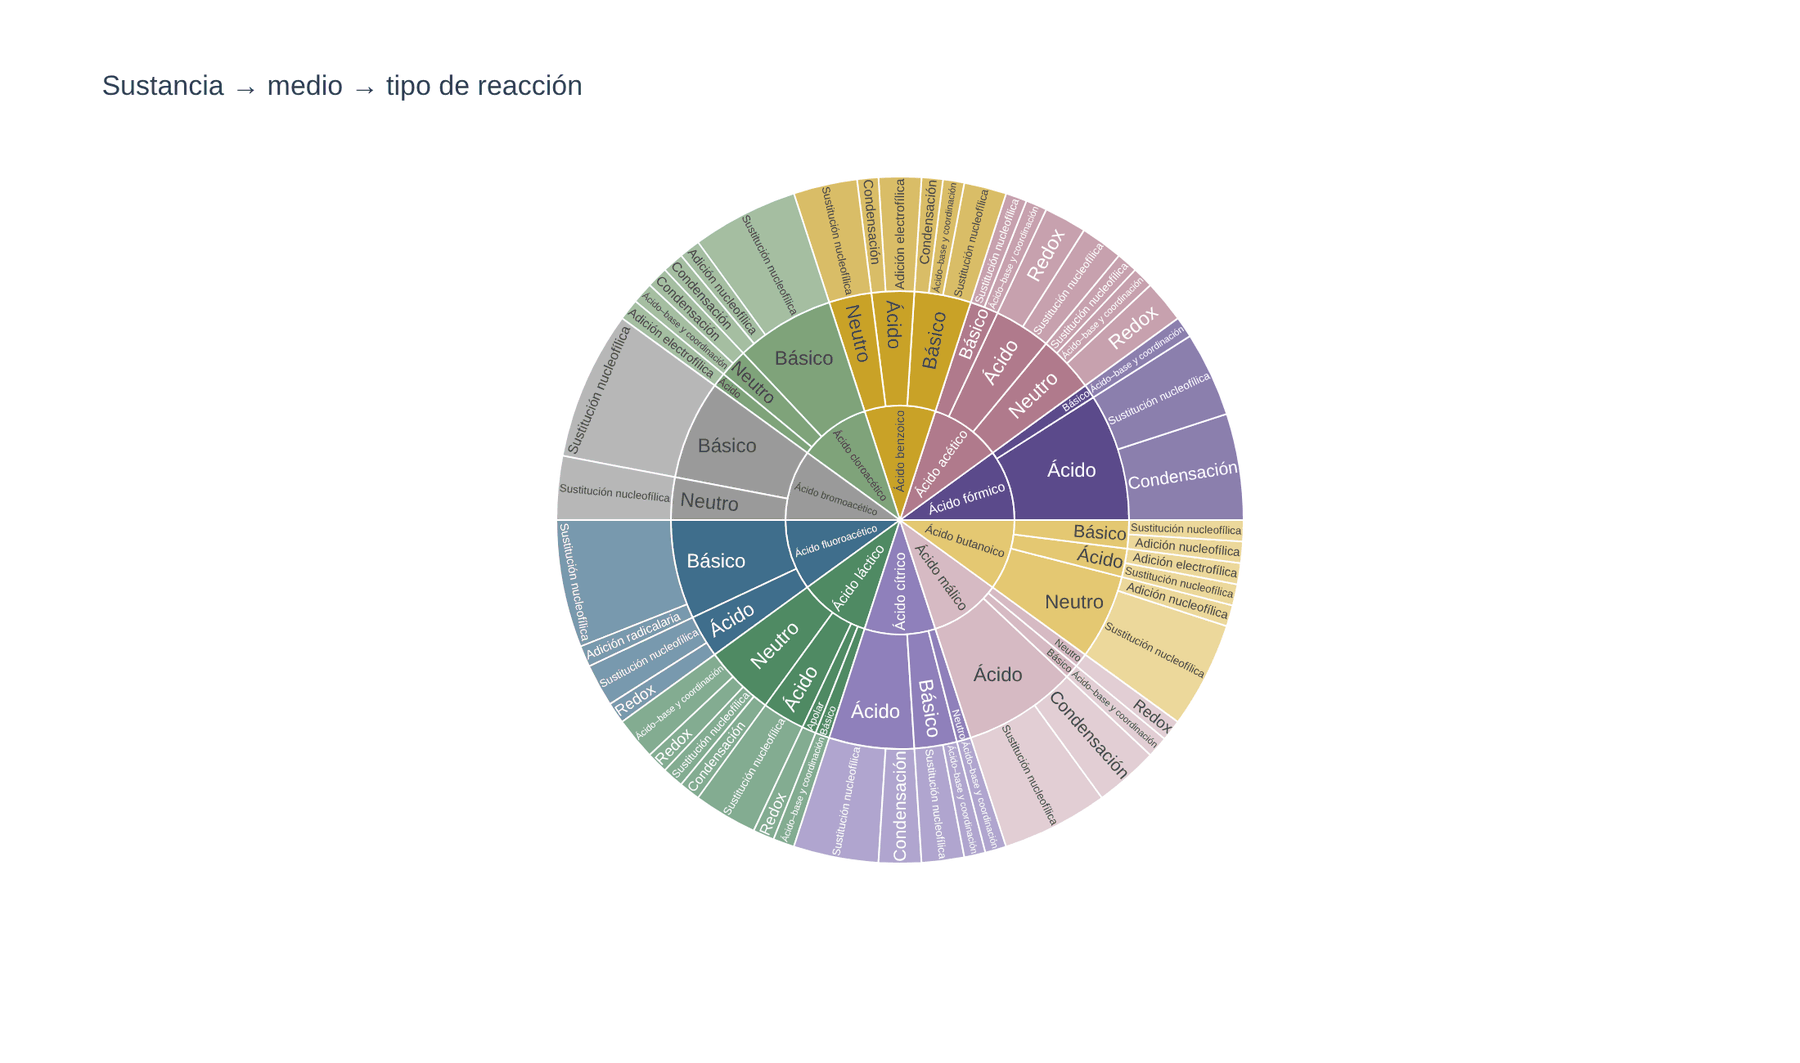
\includegraphics[width=\linewidth]{19_interactivo_solar.png}
\caption{Diagrama solar sustancia $\rightarrow$ medio $\rightarrow$ tipo.}
\end{subfigure}
\caption{Capturas de las gráficas interactivas elaboradas con Plotly (disponibles como archivos .html).}
\label{fig:interactivas}
\end{figure*}

\subsection{Limitaciones}
Cada sustancia cuenta con diez reacciones y diez obtenciones, elegidas según los resultados de la búsqueda en SciFinder. Algunos ácidos contaban con mucha información, lo que permitió seleccionar los registros más completos; para otros, el número de reacciones y obtenciones disponibles era muy reducido, en muchos casos casi igual al requerido, por lo que no fue posible filtrar los datos y los resultados pueden estar sesgados.
\FloatBarrier
\section{Conclusiones}
\fontsize{12}{14}\selectfont
En los diez ácidos carboxílicos estudiados, el tamaño molecular controla las propiedades de volatilidad: en los productos, el punto de ebullición aumenta 1.19~\textdegree C por cada g/mol ($R^2$ = 0.83) y la presión de vapor disminuye con el punto de ebullición, mientras que la densidad depende de los heteroátomos y no del peso molecular. 
La reactividad de los ácidos se concentra en la sustitución nucleofílica (58\,\% de las reacciones), sobre todo en el carbono del acilo, y su obtención se basa en procesos redox (51\,\%) e hidrólisis.
Los medios ácido y básico son los más frecuentes, y obtener los ácidos requiere calentamiento con mayor probabilidad que transformarlos.


\section{Declaración}
\fontsize{11}{13}\selectfont


\textbf{Contribución de los autores:} Integrantes 1 y 2: creación del cuaderno de Google Colab. Integrante 3: redacción del documento en \LaTeX. Integrante 4: tablero en Power BI. Todos contribuyeron a la construcción de la base de datos y revisaron y aprobaron el documento.

\textbf{Disponibilidad de datos y código:} La tabla de datos y el cuaderno de Google Colab se encuentran en el repositorio de GitHub del grupo.

\printbibliography

\end{document}